%%
%% DOCUMENT TYPE
%%

% general options:
% - inputenc        file encoding (should be "utf8" in most cases)
% - de/en           language of your work (influence pre-defined tokens)
% - declaration     adds the mandatory statutory declaration for theses
% - abstract        adds the abstract (from file "prelude_abstract.tex")
% - acknowledgment  adds an acknowledgment (from file "prelude_acknowledgment.tex")
%                   it is a nice gesture to personally thank people who
%                   supported you during your work.
% - symbollist      adds a list of symbols (from file "prelude_symbols.tex")
% - figurelist      adds and automatically creates a list of figures 
% - tablelist       adds and automatically creates a list of tables
% - index           generates an index based on the package "makeidx", please
%                   refer to its documentation for usage on index markup
% - bibbacklinks    adds backlinks from bibliography to the pages, where the
%                   corresponding entry is used (cited)
% - gray            make a gray-style version of the thesis report
%
% PhD thesis specific options
% - cv              adds your cv
% - publishsize     changes the page size from A4 to A5 for print publishing
%                   (please change the font size to 9pt, if you use this option)
% - approved        use this option, after your thesis has been formally approved
%                   (this will change the front page to meet formal/legal requirements)
% - ownpub          adds a second bibliography (from file "ownpub.bib") for your own
%                   publications related to the PhD thesis. According to the latest
%                   examination regulations, own work should be part of the regular
%                   bibliography (this option is hence obsolete)

\documentclass[en,acknowledgment,inputenc=utf8]{tuhhthesis} %symbollist taken out since there will be not many formulas
%%%%% For this projektarbeit
\usepackage{siunitx}

\usepackage[final]{pdfpages}
\usepackage{pgf}
\usepackage{tikz}
\usepackage[utf8]{inputenc}
\usetikzlibrary{arrows,automata}
\usetikzlibrary{positioning}


\tikzset{
    state/.style={
           rectangle,
           rounded corners,
           draw=black, very thick,
           minimum height=2em,
           inner sep=2pt,
           text centered,
           },
}

%%%%%%
\setthesistype{projectwork}
\author{Juan Carlos Reyes Andrade}
\title{Development of an embedded communication hub for sensor data acquisition in a robotic system}
\institute{InstSmartPort}
\submitdate{30.09.2020}
\matrnumber{21863765}
\course{Information and Communication Systems}
\examinerFirst{Prof. Dr.-Ing. Bernd-Christian Renner}{Research Group smartPORT\newline Hamburg University of Technology}
\supervisorFirst{MSc. Jannick Brockmann}{Head of Electronics at Han's Robot Germany GmbH}





%    


%%
%% CONTENT AREA
%%

% mathematical symbols
%% absolute value, ceiling, floor
\newcommand{\abs}[1]{\left|{#1}\right|}
\newcommand{\floor}[1]{\left\lfloor{#1}\right\rfloor}
\newcommand{\ceil}[1]{\left\lceil{#1}\right\rceil}

% regular sets %
\newcommand{\setN}{{\mathbb N}}
\newcommand{\setZ}{{\mathbb Z}}
\newcommand{\setQ}{{\mathbb Q}}
\newcommand{\setR}{{\mathbb R}}
\newcommand{\setC}{{\mathbb C}}
\newcommand{\classNP}{{\cal {NP}}}
\newcommand{\classP}{{\cal {P}}}

% a node and a sink
\newcommand{\node}{v}
\newcommand{\sink}{\node_{0}}          % sink

% Node Related Sets
\newcommand{\Network}{G}
\newcommand{\setNodes}{{\mathcal V}}% set of nodes
\newcommand{\setLinks}{{\mathcal E}}% set of edges
\newcommand{\setNeighbors}[1]{{\mathcal N}_{#1}}% neighbors
\newcommand{\setTree}{{\mathcal T}}% tree
\newcommand{\setChildren}{{\mathcal C}}%
\newcommand{\setLeafs}{{\mathcal F}}%
\newcommand{\numNodes}{N}%
\newcommand{\numChildren}{C}%

% density
\newcommand{\nodeDensity}{\varrho}

%% EOF


\begin{document}


% The Chapters
\chapter{Introduction}

%% Proposed roadmap
%
%   The use of RT in the industrial environments
%   Current standards IEEE and IEC and the TSN
%           Roadmap of standards
%           RTE protocols and OPC UA   
%           How are they related
%  
%   -----------State of the art--------------------------------
%   Applications with RTE and OPC UA in Hard Real Time applications     
%   A brief overview about the RT tools in robotics
%           The importance of EtherCAT as an open RTE protocol within robotics
%   Comparison of openess
%   EtherCAT introduction (selected by Hans Robot)
%           Focus on EtherCAT XoE <<THIS ONLY NEEDS TO BE MENTIONED
%------------------Out of scope--------------------------------------
%   HW ASICS and stuff like that
%   SW Stacks for EtherCAT development and other RTEs
%
%

% Terms:
% ACB = Axis communication board, alias for embedded communication hub for sensor data acquisition in a robotic system
% RTE = Real-Time Ethernet as specified in IEC 61784-2:2019. \cite{rte:standards}
% IIoT = Industrial Internet of Things

% 95/100
This document describes the different stages through the development of an embedded communication hub for sensor
data acquisition in a robotic system, within dis document this prototype will be refered as \emph{Axis Communication Hub} or ACB. 
During this chapter a brief introduction to the Real-Time Ethernet (RTE) industrial networks is presented, as well as 
a summary of the standards involved with comments about how they are related to each other. Moreover, the usage of these RTE 
industrial protocols in embedded applications and its relation to the Industiral Internet of Things (IIoT) necessities is 
briefly introduced. Finally in this chapter, a brief comparison of the openess of these protocols and how this is related 
to the development of devices is presented. 
The second chapter shows a summary of the state of the art regarding the possibilities for developing open source projects 
according to the degree of openess of an RTE communication protocol. This has focus on EtherCAT devices as it is within the 
scope of this Research Project and shows advantages that will be detailed as the reader reads through this document. 
Afterwards, the third chapter deals with the goal of the Research Project and its proposed solution. 
a summary of technical specifications, the hardware available, software structure and an overall prioritization of the goals
is also included. 
Later on, during the fourth chapter, the main points related to the implementation is presented. 
The overall results are discussed in chapter five, where the reader can find comments about the implementation and test 
challenges. As part of the conclusions chapter, a proposed list of points for further development is discussed. 
Finally, extra information focused on the technical details of the implementation can be found within the appendixes.

\section{The need of RT within industrial environments}

%90/100
During the last years an increase in the usage of the Ethernet-based fieldbuses within industry has been recorded. This, with no surprises,
shows the expected adaptation of the industrial automation to the IT infrastucture, which is fundamental for the \emph{Industrie 4.0} paradigm
and its consequent huge amount of data to be monitored, analyzed and controlled, dealing at the same time with differnt time constraints and
interconnectivity among the different layers of an industrial system and their devices. 
Having in mind the current \emph{automation pyramid} with direct access from the top to the bottom\cite{tsn_intro}, see figure \ref{fig:pyramid-iiot}, 
it is understandable that several technologies providing this access have been meeting each other comming either from the top or the down levels, 
at the point that they offer similar features regarding data access and security. Each of them with their own development history,
alliances and, therefore, standards. Comming from top-level-related frameworks there is, e.g., the OPC UA project; whereas names like Profinet,
DeviceNET, EtherCAT, Powerlink, etc, come from the fieldbus side -lowest level-. All of them have developed in an individual way as response
of market, however meeting in the late decade through the necesity for unified standards to improve interoperability between the incredible number
of projects. This happens at a time were information, technical as well, and development tools have become even more available and
open to the end-user. Leading now then to a situation where the private initiatives are not any longer the full owners of the technology development.

\begin{figure}[b]
    \centering
    \includegraphics[width=.5\textwidth]{imgs/intro-industryarchitecture.jpg}
    \caption{\emph{Industrie 4.0} architechture. Industrial Internet of Things.\cite{tsn_intro}}
    \label{fig:pyramid-iiot}
\end{figure}

Another line of work, closely related to interoperability, is the Real Time (RT) applications in their both versions with \emph{hard} and \emph{soft} requirements. 
Nowadays, there is an increasing number of applications in robotics that demand control loops and device chains that
demand hard real time performance. Although, this requirements are more typical at the device level, such as, robots, cncs, etc. They all now face 
the IIoT requirements; hence, their networks should meet as well certain degree of RT capability. Moreover, synchronization of time sensitive
systems within manufacturing lines, for instance, has been addressed for years by the RTE protocols and now these sort of features are increasingly
been demanded as well at upper levels IT levels.



\begin{figure}[ht]
    \centering
    \includegraphics[width=\textwidth]{imgs/intro-buses-share.jpg}
    \caption{Industrial network market shares 2020 according to HMS Networks.\cite{fieldbus_shares}} %Add the reference, this could be a table
    \label{fig:fieldbus_shares}
\end{figure}

The current automation industry has a record of many competitors and closetechnologies, as natural consequence for specific processes requirements (depending on the industry), 
but also as a response of market strategies. Nevertheless, the serach for standardization
can be tracked back to the $80$s, as the fieldbuses were standardized by the International Electrotechnical Commission (IEC). 
Continuing after the Ethernet took its place within the industry. As an important note, during the last two years, according to the HMS Industrial Networks' annual study,
the total market shares of new industrial nodes in factory automation increased for the Industrial Ethernet from $52\%$ to $64\%$; as the commonly called
fieldbuses decreased in the same period from $42\%$ to only $30\%$; finally the industrial wireless remained around the $6\%$, see figure \ref{fig:fieldbus_shares}. \cite{fieldbus_shares}

It is yet worthy to mention that the name \emph{Industrial Ethernet} is used only as a 
generalization for the group of protocols that historically developed on IEEE's Ethernet specification; even though, they all are almost no further
compatible with each other -as they have modified Media Access Control (MAC) Layers-. More details about this differences will be addressed in the following chapters.  

%95/100
As history shows, vendor protected technology have its limit when there are plenty of possibilities for automation technologies, even if they are in ongoing development. 
For instance, as happened during the lifetime of the Open Platform Communications OPC -predecessor of OPC UA-, that was started only upon \emph{Microsoft Windows} and 
as the time went by, the emerging needs made it change to use open standards and a multiplatform approach.

To introduce the reader to a common ground regarding standardization, the following chapter will present a brief summary of the standars that 
are of interest for anyone who wants to start developing using industrial interfaces.

\section{Industrial standards and the TSN initiave}\label{sec:standards} 
%97/100
This section is intended to provide the starting developer a rough but useful reference of the standards related to industrial 
communication networks. If the reader has already good knowledge of these standards, this section can be easily skipped and continue 
with the next chapter.
First of all, due to the historical and technological process of innovation within the information and communication 
systems, several parties have been related and, at some extention have merged results, bringing out an interconnected 
set of norms that thrive continuosly onto a global standardization.

The following list is intended to be a quick reference to the current standards for Ethernet, legacy and current fieldbuses, 
Time-Sensitive Networks in their american and international iniciatives. This way, the reader has a roadmap to be taken into
account for deeper research within the industrial applications. 
Furthermore, information related to the similar standardization processes between 
the IEC, ISO and IEEE, and their unavoidable cooperation, can be read in \cite{standards_coop}. %a comparisson of the ieee and iec standars processes

\begin{description}
    \item[ISO/IEC/IEEE 8802-3:2015] Revision of the Ethernet standard for half and full-duplex communication up to $100Mbps$. Originally
        published by american IEEE 802-3 in 1985 and accepted internationaly in 1989. The last revision 8802-3-2017/Amd 10-2019 includes
        MAC controls for 200 and 400 Gbps.\cite{iso8802_ethernet} %https://www.iso.org/standard/72048.html 
        After 2019 The name Ethernet is not longer used, instead CSMA/CD or a reference to the corresponding ISO standard 8802.3 is the formal name.
    \item[IEC 61158:1999-2000] First international fieldbus standard published in 1999, where 8 \emph{Types} of fieldbuses were introduced addressing the 
        Physical Layer (PhL), the services and protocols of Data Link Layer (DLL) and Application Layer (AL). Some included brand 
        names were the following: H1/HSE/H2, ControlNet, EtherNET/IP, Profibus, Profinet, Interbus. This standard has an interesting story
        concluding with the signing of the \emph{Memorandum of Understanding} by the main contenders to put end to the fiedlbus war.\cite{fieldbus_history} %The Fieldbus Standards: History and Structures
        Its most updated version in 2019 counts with 26 Types of protocols and grouped them as fieldbus Communication Profile Families (CPF). 
    \item[IEC 61784-Part 2:2008] It is an extension for the CPs capable of RT that are based on the IEEE 8802-3 standard (commonly named Ethernet). Commercial names included 
        are the next: EtherCAT, Profinet, Ethernet/IP, Ethernet Powerlink, and Modbus TCP.\cite{future_iiot} %Industrial Communication Systems and Their Future Challenges: Next-Generation Ethernet, IIoT, and 5G
        The SERCOS CPF is highlighted, since its third version is, altogether with the EtherCAT profile, the fastest one in the list; providing as well
        a more efficient use of the available bandwidth with an open source resources. IT shows even advantages over CAN devices due
        to its original design intended for hard RT motion control.\cite{sercos_origin}\cite{sercos_performance} %https://www.designnews.com/sercos-picks-pace %https://www.sercos.org/technology/advantages-of-sercos/performance/. 
        This is a very interesting Hard Real Time capable protocol that might need further development which is not included in the scope of this 
        Research Project.
    \item[IEEE 802.1A/B/C/D/Q] Time-Sensitive Networking standards is an initiative to improve the IEEE 802-3 in order to meet the industrial real time requirements, 
        which story can be tracked back to 2005, as the IEEE 802-3 group was merged with the IEEE 802.1 Audio Video Bridging Task Group and started to work for
        industrial environments. This a response to the vast alternatives of the RTE CPs. About 60 individual IEEE standards oriented to improve
        the ISO/OSI layer 2, including 13 focused on its security, are within the scope of the TSN project. \cite{future_iiot} %section about the TSN
        The mentioned project covers the lower layers of the communication system, whereas the upper ones, representation and transfer of data, is
        addressed by OPC UA. Moreover, it is important to mention that this is an on-going project and still around $40\%$ of its standars are
        in draft or preparation phase.\cite{tsn_homepage}
    \item[IEC/IEEE 60802] TSN Profile for Industrial Automation is the stand alone TSN base standard that will include the common advancements
        from IEC SC65C/WG18 and IEEE 802 work groups mentioned in the previous item.\cite{tsn_profile}%https://1.ieee802.org/tsn/iec-ieee-60802/
        This is an on-going project started around 2017, still being in a draft phase. Since this will be the international standard, it would be 
        the equivalent to the effort once given during the creation of the IEC 61158 for the legacy fieldbuses.
    \item[IEC 62541:2016-2020] Set of IEC standards for OPC UA. Individually, the IEC 62541-14:2020 defines the OPC Unified Architecture 
        (OPC UA) PubSub communication model. It defines an OPC UA publish/subscribe pattern which complements the client server pattern defined 
        by the Services in IEC 62541-4. IEC TR 62541-1 gives an overview of the two models and their distinct uses.\cite{opcua_standard} %https://webstore.iec.ch/publication/61108  
        Quoting: \emph{OPC UA is a client-server communication protocol for industrial use cases without hard realtime requirements. The new PubSub 
        extension of OPC UA adds the possibility of many-to-many communication based on the Publish / Subscribe paradigm. 
        In conjunction with the upcoming Time-Sensitive Networking (TSN) extensions of Ethernet, OPC UA PubSub aims to also cover 
        time-deterministic connectivity.}\cite{opc_tsn_application} %Open Source OPC UA PubSub over TSN for Realtime Industrial Communication
\end{description}



% CANopen protocol is not capable of hard real time capabilities?


% >>Here comes information about SERCOS. The SERCOS interface started as a project for providing a Hard Real Time capable communication
% bus, it has been developed during the years, having nowadays three versions. The first ones operating over a serial bus and submitted
% to the IEC, which in 1995 released it as IEC 61491.[2] After the release of the original standard, original working group member companies 
% including ABB, AEG, AMK, Robert Bosch, Indramat, and Siemens founded the "Interest Group Sercos" to steward the standard. \ref{dummy} %https://en.wikipedia.org/wiki/SERCOS_interface#cite_note-3
% Even though the capabilities meet hard real time requirments, compared to other technologies, is rather limited. %https://en.wikipedia.org/wiki/SERCOS_interface#cite_note-3
% For the last version it has been capable to address up to 60 Motion Axes and makes use of the Ethernet standard, making it an alternative
% for the mentioned technology comming from BEckhoff. Together with EtherCAT, Sercos is the fastest 100Mps industrial Ethernet technology.
% One advantage so far of this protocol is its parallel development with the OPC UA, making it natively compatible with such networks* 
% and security layers.



\chapter{State of the art}\label{cha:state}

%% Proposed roadmap
%
%   The use of RT in the industrial environments
%   Current standards IEEE and IEC and the TSN
%           Roadmap of standards
%           RTE protocols and OPC UA   
%           How are they related
%  
%   -----------State of the art--------------------------------
%   Applications with RTE and OPC UA in Hard Real Time applications     
%   A brief overview about the RT tools in robotics
%           The importance of EtherCAT as an open RTE protocol within robotics
%   Comparison of openess
%   EtherCAT introduction (selected by Hans Robot)
%           Focus on EtherCAT XoE <<THIS ONLY NEEDS TO BE MENTIONED
%------------------Out of scope--------------------------------------
%   HW ASICS and stuff like that
%   SW Stacks for EtherCAT development and other RTEs
%

This chapter introduces some current applications mainly focused on robotics, since this area is closely
related to the environment with which the ACB will be interacting. Robotics sees various advantages
from the RT communication protocols, when it comes to integrate motion controllers and 
any other industrial peripheral. Afterwards, an overview about industrial development frameworks is 
given, yet focused not on the RT interfaces, but its specific software. The latter is of great importance,
for the Real Time Operative Systems (RTOS) are a corner stone for embedded systems that need to provide a 
deterministic service within their environment.


\section{Current applications}\label{sec:applications}

As rapidly mentioned in Sect.~\ref{sec:standards}, the SERCOS motion control interface has been standardized within the 
CPFs of IEC 61784-Part 2. Furthermore, it has been even integrated to EtherCAT as a compatible CP. 
This service is available within the DLL and AL and is called Servo Drive Profile over EtherCAT  (SoE), 
which provides access to motion controllers under 
the SERCOS specifications and, consequently, offers interoperability within its own RT features and the latter's hard RT 
capabilities.  
An example of this compatibility is presented in ~\cite{ecat_sercos}, %Motion Control System using SERCOS over EtherCAT
it shows that jitter of 30 microseconds is feasible in a control loop while the Master uses the SoE service.

Another interesting application has been the characterization of an EtherCAT Master within a RT control 
loop for Servo Motors, which run CAN devices over EtherCAT (CoE service). The implementation of the Master 
device ran on different open source Real Time Operating Systems (RTOS) based on Linux, 
namely, Xenomai and Linux with the \emph{RT\_PREEMPT} patch. It was concluded that both of the approaches 
were capable to achieve update periods of \SI{1}{\milli\second} 
, and an average jitter of \SI{1.5}{\micro\second}. Moreover, Xenomai could averagely achieve execution times around \SI{100}{\micro\second}; 
the mentioned data can be reviewed in ~\cite{ecat_xenomai}.%Real-time Servo Control using EtherCAT Master on Real-time Embedded Linux Extensions. 
It is worth to mention that the EtherCAT Master features were available in both RTOS kernels, 
for the IgH EtherCAT Master stack was running on top of them. This open source stack will be commented in ~\ref{sec:openness}.

The characterization and optimization of performance for different RTE profiles within TSN is a currently expanding topic, 
as the TSN standards and the RTE commissions are still working together. In ~\cite{tsn_and_sdn} %Integrated Industrial Ethernet Networks: Time-sensitive Networking over SDN Infrastructure for mixed Applications
are presented simulations of TSN topologies with EtherCAT and SERCOS data frames, where the Quality of Service (QoS) 
is addressed and evaluated through the usage of Software-defined Network (SDN) switches. 
The approach of this project is to test different scheduling features given fixed cycle times for the data frames, 
which were proposed to be similar to the current real industrial applications
in both technologies. In this manner, the importance of an unified network that supports different protocols is highlighted, 
but further research in this topic, including tests with other RTE data frames are still to be researched.

Besides robotics, a recent industrial application concerning CBD extraction equipment for high-performance large-scale processing,
implemented distributed control and monitoring based on EtherCAT open protocol. This article can be seen in ~\cite{ecat_industrial}.

Addressing the usage of open source tools, such as OS and RTE Protocols, for development of complex robotic systems, in ~\cite{ecat_motionplanning} %Motion Planning for Quadrupedal Locomotion: Coupled Planning, Terrain Mapping and Whole-Body Control
is presented a \emph{Motion Planning for Quadrupedal Locomotion}. This is roughly composed, besides the hydraulic actuators, mechanics and other peripherals, of two PCs on board with RT capabilities and shared memory. 
RT Linux (Xenomai) runs on both of them and take care of different levels of the control threads at two different rates depending on the tasks, 
namely \SI{1}{\kilo\hertz} and \SI{250}{\kilo\hertz}. The former rate is used
for communicating with the motor controllers over EtherCAT interfaces.

Currently, Han's Robot Germany GmbH focuses on enhancing robots’ cognitive abilities by developing in the fields of environment perception, 
drive technologies, 
control theory, material science, mechanical design and artificial intelligence. Interfaces within the robotic system rely on various
industrial protocols to make its interoperability one of the key features. For instance, current motor drivers
are linked over internal EtherCAT chain to the main controller.

The above mentioned applications are just a tiny number of examples that shows the importance of an already standardized open industrial communication protocol, 
within a broad set of fields that cannot be completely covered in the scope of this document. Nevertheless, it paves the road to understand why generating the know-how 
to any of the mentioned technologies, represents a high-impact resource for any research or development group, regardless of its commercial or academic purposes.

\section{An overview about the RT capable SW in robotics}

As mentioned in the previous section, several resources and examples showed the current usage of RT
open source software and its community. Since this Research Project has a goal of introducing the reader a 
roadmap for RTE communication interfaces and 
its applications, this section was added to summarize the RT software for development in robotics.

The usage of middlewares within the field of robotics is growing and it relies on \emph{robot software} that 
exists between the application and an RTOS, as detailed in the following articles ~\cite{ecat_xenomai} and ~\cite{ecat_motionplanning}.%the robot examples.

A list of requirements is suggested in ~\cite{middleware_industrial} %2020-Real-Time Robot Software Platform for Industrial Application 
to address the mentioned middlewares and how to consider them \emph{Real Time Robot Software Platforms}.  
The list is as follows and it is useful to start getting familiar with the capabilities 
and features of the so-called Robot Software: 
\begin{enumerate}
    \item Data exchange support.
    \item Real time support (strict periodic execution and sporadic events support).
    \item Thread and process types for user defined programs support.
    \item Easy configuration of applications (robot control SW, PLC SW, vision inspection SW, non-real-time SW, etc.)
    \item Multiple periods for scheduling.
    \item Threads or processes running in the same period are classified by priority.
    \item Check and handle the event through the event handler.
\end{enumerate}

Common names for different projects aiming to create these development frameworks are the following: Common Object Request Broker Architecture
(CORBA), Real-Time CORBA (RT-CORBA), Data Distribution Service (DDS), OPC UA, Open Platform for Robotic Services (OPRoS), 
Open Robotics Technology Middleware (OpenRTM), Open Robot Control Software (OROCOS), 
and Real-Time Middleware for Industrial Automation devices (RTMIA). Further comments and a comparisson between their features
can be seen in the previously referenced paper. As to what concerns to this document, only some of them will be roughly commented
as they ended up being somehow related to the RTE profiles. For more information review ~\cite{middleware_xbotcore}.

\begin{description}
    \item[OPC UA] As frequently mentioned before, this is an open standard for data sharing among nodes within industrial networks and has
    been considered in some projects related to robotics. Nevertheless, it is important to highlight that this is not considered a full 
    middleware, since it only provides a protocol to control the exchange of data between nodes, a good degree of reliability and security.
    However, it does not provide RT capabilities to the system only compatibility. Hence, it needs an operative system and the consequent 
    lower layers capable of RT scheduling and communication, concerning the latter the TSN set for protocols is an example.
    \item[ROS/OROCOS/OpenRTM] These are projects that aim to create a suitable middleware for robots by implementing Xenomai or Linux operating systems. 
    ROS prioritizes the final user, avoiding in the way some fine-grained features due to its difficulty, therefore having sometimes
    issues to meet the hard RT requirements. Whereas OROCOS has further improved its compatibility, similarly to OpenRTM.
    \item[CODESYS and TwinCAT] To fully meet compatibility with the industry, the so-called PLC Software has been also used in open robotics.
    These applications essentially need to run both, the robot functional blocks and the robot tasks. For further details on it the following
    references can be reviewed ~\cite{middleware_xbotcore} and ~\cite{middleware_xbotcloud}. %referemces from the italian robot Xrobotcore
    \item[xbotcore] This is an attempt to provide of a highly compatible open middleware for industrial robotics, it runs over the Xenomai and 
    uses a SOEM stack to interface with any compatible industrial device, recall ~\ref{sec:openness}. % XBotCore: A Real-Time Cross-Robot Software Platform 
    Applications have been already mentioned in ~\ref{sec:applications}, which have reached control loops down to 1khz for 33 axes. More details about the 
    latter application in ~\cite{middleware_xbotcore}.
    %\item[RTMIA] RTMIA middleware + Linux or Xenomai but used open PLC running parallely[?] << This needs further reading [?]
\end{description}


The previous information was presented only to draw an idea for the non-familiar reader about the applications and, since this topic is in ongoing development 
and, furthermore, many other platforms are addressing similar challenges; the reader is invited
to go deeper into these topics, for instance, by reviewing this resource ~\cite{middleware_industrial}. %add the resouce fromt he open community 

\section{Approaching openness within the RT protocols}\label{sec:openness}

Among the industrial standards mentioned in ~\ref{sec:standards}, there are some related initiatives to include a certain degree of open source
software to improve the development of applications. The following is a brief list of a few interesting references to them. 
However, as expected, most of the software stacks
for industrial communication systems are commercial and provided by third-party companies. 

%90/100
\begin{description}
    \item[OSADL] Open Source Automation Development Lab eG (OSADL):It is a German group that intends to lead the development of open source development
    for industrial automation. Closely related in the developing of OPC UA and other Linux features for industrial applications.
    \item[open62541] Within the official scope of OPC UA, there is this Certified SDK project that is within its second phase, at which it is expected 
    from the research and industrial community to develop applications to test its performance. Moreover, as the TSN specification is of huge importance, 
    a set of enhancements for the open62541 project were developed by Fraunhofer IOSB and series of patches for the Linux kernel have been released to 
    make it an RT compatible. To review the overview of the project, visit ~\cite{open62541_homepage}. %https://www.osadl.org/OPC-UA-over-TSN.opcua-tsn.0.html 
    The OPC UA is developed under GPL 2.0 license and due to its current phase implies a further adaptation for the physical node, e.g., ARM arquitechtures 
    to make them compatible with the mentioned patches. 
    \item[SOEM/SOES] RT Labs Industrial development group focused on Software Stacks for industrial protocols. Among their commercial communication stacks
    there are software stacks under GPL for EtherCAT Master and Slave devices SOEM/SOES. More details about these stacks can be found in ~\cite{soesm_homepage}. %https://rt-labs.com/product/soes-ethercat-slave-stack/ 
    \item[Sercos Stacks] Sercos III technology is able to be operated in a common TSN-based network, % Ethernet TSN heralds a new era of industrial communication
    since its development group has been working closing together with the TSN group; a more detailed scope can be seen in ~\cite{sercos_tsn}. 
    They also made available open source software dedicated for development of master and slave devices, namely: Common Sercos Master API (CoSeMa),
    Sercos Internet Protocol Services (IPSS), and The Sercos III SoftMaster, the latter even allows the host to use any standard Ethernet controller. %https://www.sercos.org/technology/implementation/driver-software/. 
    It is important to mention that there are testing tools to certificate those devices and achieve a Safety Integrity Level 3 (SIL-3). A description of the
    different available libraries is provided in ~\cite{sercos_stacks}.
    \item[EtherNet/IP Stacks] There are several commercial stacks that comply with the Open DeviceNet Vendors Association's (ODVA) EtherNet/IP specification. 
    OpEner is an open source alternative which targets PCs with a POSIX operating system and a network interface. 
    Integration examples are provided only in Linux and Windows in ~\cite{opener_stack}; %http://eipstackgroup.github.io/OpENer/index.html
    nevertheless, a variation for embedded systems has been presented for an STM32 microcontroller. In the mentioned project, more tools had to be adapted, for instance,
    STM32F4x7 Ethernet Driver v1.1.0, lwIP v1.4.1 (TCP/IP Stack), MicroHTTP v5.1.0.1, a patched version of OpENer v1.2., among others. A detailed description
    of the requirements can be reviewed in ~\cite{opener_stm32}%https://www.emb4fun.de/archive/chibiosopener/index.html
    \item[IgH EtherCAT Master] This is a bundle of libraries to give a Linux host (LinuxCNC for example) EtherCAT Master features, it is developed under the GPLv2 license. 
    An interesting example of this open source resource within an Airbus Test Rig can be reviewed in the following reference ~\cite{ecatstack_igh}. %https://etherlab.org/en/success/airbus-testrig.php
\end{description}

As the scope of this Research Project is only focused on the industrial communication profiles capable of RT and, so far has been clear how 
the EtherCAT is a reliable one, yet open and significantly considered in the industry ---recall Sect. ~\ref{sec:applications}. 
Hence, it makes sense to invite the reader to read the introduction to the protocol itself in the Appendix ~\ref{sec:ecat_protocol}. 
This way it is easier to go sensibly to the implementation of what is one of the basic chain-elements in what could become a very complex application: 
an EtherCAT Slave device with open source elements.


\chapter{Design requirements and approach}\label{cha:solution}

This chapter presents the main goals of the project and the technical specifications. It is also 
intended to give the reader a summary of the proposed functional modules and its structure. 
Any other constraint not mentioned here 
was adjusted or set while being within the design-test loop, as consequence of the prototype nature of the project.
\section{Objectives}
The main goal of this project is to develop a device using open-source tools to read out sensor data from a robot
axis that can be interfaced with an RTE Network. Such that this device can be used afterwards as a test platform 
within an industrial environment to characterize its compatibility with the ongoing IEC/IEEE 60802
TSN Profile for Industrial Automation.

To achieve the main goal the following has to be carried out:
\begin{itemize}
  \item To specify the requirements of the system
  \item Comparison considering the state of the art
  \item To develop the embedded system as a functional EtherCAT Slave Device
  \item To design and manufacture a PCB prototype
  \item To test and report the overall system functionality
\end{itemize}

\section{Technical specifications}

In the table \ref{tbl:tech_specs} the requirements for this project and their state after the implementation can be observed.
This comparison helps as a good summary of the overall achievements that are further detailed in the next chapters.

  \begin{tuhhtable}
    \footnotesize\centering
    \begin{tabular}[hbp]{L{.22\textwidth}L{.22\textwidth}L{.22\textwidth}L{.22\textwidth}}
        \THc{1}{c}{Feature} & \THc{1}{c}{Requirement} & \THc{1}{c}{Implementation} & \THc{1}{c}{Remark} \\
      \abovebodyrule
      \TRh{1}{l}{Upper layer interface}  & Ethernet/EtherCAT compatibility.\newline Non-safety relevant.\newline Services and synchronization: - 
                                        & EtherCAT slave.\newline Services: Mailboxing and CoE\newline Synchronization: Free Run and SM  
                                        & \tblYes\newline FoE and SD synchronization possible in the medium term.\\\TRc
      \TRhc{1}{l}{Display/signaling}    & LED stripes with serial interface:\newline WS2812 \newline 2 Ch  
                                        & 2-4 Ch modifiable in SW\newline Animation capable 
                                        & \tblYes\newline Chs can increase up to number of DMA-Timers (8)   \\
      \TRh{1}{l}{Temperature}           & Data interface for 1-Wire bus     
                                        & 1-Wire Master\newline 15 sensor in bus & \tblYes\newline 6 Sensors simultaneously tested \\\TRc
      \TRhc{1}{l}{PCB}                  & PCB Prototype\newline Layout and size: -   
                                        & Attachable PCB for LAN9252-EVB-SPI.\newline Size: \SI{55 x 38}{\milli\metre} & \tblYes\newline Second layout with both chips included possible in the short term. \\
      \TRh{1}{l}{Safety}                & \tblNA     
                                        & Non Safety-Critical for this prototype & \tblNo\newline FSoE could be researched in the long term.\\\TRc
      \TRhc{1}{l}{Extra interface}      & SPI or I2C interface for current/IMU/black channel   
                                        & Extra SPI considered in PCB and SW\newline JTAG/SWD compatible interface & \tblYes\newline Currently working \\
      \TRh{1}{l}{Speed/position}        & Possible interface of BISS-C type
                                        & Not required for this prototype & \tblNo \\\TRc
      \TRhc{1}{l}{Refresh data cycle}   & -   
                                        & No hard RT deadlines.\newline Deterministic refresh cycle of $\sim$\SI{10}{\milli\second} by RTOS.\newline Timeout faults handling. & \tblGood\newline Timing through RTOS  \\
      \TRh{1}{l}{Data structure}        & -     
                                        & Functional and parametrization data structure as Object Dictionary.\newline Standard ESI file. & \tblYes\newline Currently working\\\TRc
      \TRhc{1}{l}{FW programming}       & -   
                                        & CMSIS - FreeRTOS for thread, event and time management. & \tblGood\newline Currently working \\
      \belowbodyrule
    \end{tabular}
    \caption{Technical specifications;}
    \label{tbl:tech_specs}
  \end{tuhhtable}

Regarding the functional safety features of the device, it is important to mention that, even though this device is considered as non Safety-Critical within
this prototyping stage, the means to create a framework that could be extended to address further reliable development are taken into account, namely
by considering fault tolerance within the software. More comments about this will be done in the results section. 

\section{Solution proposal}
In Fig.~\ref{fig:sysStruct} the proposed layered structure of the functional blocks can be seen, this will help the reader
localize how is the level of interaction of each of the parts that are described along the document. For instance, the project itself 
focuses mainly on the non-dashed blocks; nonetheless, they still need to be configured or adapted according to ACB features. The layered
representation shows three general concepts, namely physical or hardware, middleware and application software. Even though, the blocks
help the reader differentiate between functionalities, most of them are interacting between each other, mostly the Devices' State Machines (DSM).

\begin{figure}[ht]
  \centering
  \includegraphics[width=\textwidth]{imgs/prop-system_struct_v2.png}
  \caption{Layered structure of the proposed functional blocks.}
  \label{fig:sysStruct}
\end{figure}

\section{Hardware selection}

In this part it is presented the base hardware that was available to develop the prototype. The microcontroller (MCU) was chosen
due to its active community, resources and current on-develop projects. Other MCUs were though considered, since the overall characteristics
were somewhat similar and generic---regarding peripherals like serial interfaces or Direct Memory Access (DMA) and processing power and memory, for instance.
Therefore, MCUs from Infineon and 
Texas Instruments were good possible candidates---see technical information in ~\cite{infineon_esc},~\cite{infineon_dramfine} and ~\cite{texasi_esc}, respectively; 
however, the basic familiarity with the STM32CubeIDE and the related ST technology 
was a crucial factor. In addition, and concerning the chosen MCU as well, the learning curve is not negligible when it comes to develop any 
firmware at a fair level, even more when it deals with other to-learn
tasks, for instance, development with RTOS, modification of open libraries, EtherCAT protocol itself and the Network Controller chip.

Regarding the Network Controller, the LAN9252 belongs to a set of ASICs that are verified and certified by Beckhoff Automation GmbH. For a further
reference for other alternatives visit ~\cite{beckhoff_esccomparison}. The LAN9252 integrates a so-called EtherCAT Slave Controller (ESC) and it represents a good 
alternative to the Beckhoff's original ASIC ET1100. This way, the basic hardware is there to fulfill Han's Robot Germany's
proposal for developing industrial compatible devices that could enhance the prototyping process within the electronics department. 
Moreover, the mentioned ASIC has a wide compatible control interface that make it be suitable to any microcontroller with which 
the developer has experience. The Table~\ref{tbl:hardware_characteristics} lists the main characteristics of the above mentioned hardware.

\begin{tuhhtable}
    \footnotesize\centering
    \begin{tabular}[tp]{L{.44\textwidth}L{.44\textwidth}}
        \THc{1}{c}{STM32F446ZE} & \THc{1}{c}{LAN9252} \\
      \abovebodyrule
        ARM®32-bit Cortex®-M4 + FPU + Chrom-ART™ Accelerator
        Up to 180MHz CPU\newline
        512 kB of Flash\newline
        128 KB of SRAM
                                        & EtherCAT slave controller with
                                        3 FMMUs and 4 SyncManagers\newline
                                        Distributed clock support\newline
                                        4KB of DPRAM\\\TRc
        General-purpose DMA\newline
        Up to 17 timers\newline
        Up to 4 × I2 C interfaces\newline
        Up to 4 USARTs/2 UARTs\newline
        Up to 4 SPIs\newline
        2 × CAN (2.0B Active)\newline
        USB 2.0 full-speed device/host/OTG 
                                        &100Mbps Ethernet transceivers compliant with IEEE 802.3/802.3u (Fast Ethernet)\newline
                                        8/16-Bit Host Bus Interface, indexed register or multiplexed bus\newline
                                        SPI/Quad SPI\newline
                                        Digital I/O Mode\newline
                                        Multifunction GPIOs
                                        \\
        LQFP64, LQFP100 and LQFP144 packaging     
                                        & Pb-free RoHS compliant 64-pin QFN or 64-pin TQFPEP packaging 
                                        \\\TRc
      \belowbodyrule
    \end{tabular}
    \caption{Summary of the characteristics of both STM32F446ZE and LAN9252 used in the prototype.}
    \label{tbl:hardware_characteristics}
  \end{tuhhtable}

%\subfigbox{
%    \subfigure[NUCLEO-STM32F446ZE]{\label{subfig:stmboard}\includegraphics{imgs/sol-stmboard.jpg}}
%    \subfigure[LAN9252-EVB-SPI]{\label{subfig:lanboard}\includegraphics{imgs/sol-lanboard.jpg}}
%}{Evaluation boards for prototyping.}{fig:evalboards}

\begin{figure}[ht]
    \centering
    \subfigure[NUCLEO-STM32F446ZE]{\label{subfig:stmboard}{\includegraphics[width=0.4\textwidth]{imgs/sol-stmboard.jpg}}}\hfill
    \subfigure[LAN9252-EVB-SPI]{\label{subfig:lanboard}{\includegraphics[width=0.4\textwidth]{imgs/sol-lanboard.jpg}}}
    \caption{Evaluation boards for prototyping.}
    \label{fig:evalboards}
\end{figure}

\section{PCB design}\label{sec:pcb_proposal}
As it can be seen in the figure \ref{subfig:lanboard}, the evaluation board includes on-board male pins, this was taken as an advantage and the PCB to be designed
consisted on a pluggable PCB that would be mounted on top of it, increasing minimally the volume already occupied by the evaluation board. This idea needed to be 
designed taking into account the minimum of components based on the Nucleo-STM32F446ZE original design and the requirements of the LAN9252. This means that 
it had to provide, both 5V and 3.3 V power supply, physical ports for the prioritized communication capabilities, minimally SPI, One-Wire JTAG and the LED ports 
according to the technical specifications \ref{tbl:tech_specs}.

\section{Firmware structure}

Since the compatibility with the EtherCAT protocol is the highest priority, all the tasks related to the adjustment of existing libraries and 
the synchronization between them are also prioritized, such that the main functionality can operate. Taking this into consideration and 
recalling the final proposal for the structure of the embedded system, Fig.~\ref{fig:sysStruct}, the functional blocks are represented differently. 
The ones in gray or dashed lines are mainly components that are planned not to be modified
at all or not in deep, because of either its complexity or its given reliability. This means, its functionality is almost granted. 
Nevertheless, the progress relies on documentation that can be either good or poor, for instance, TwinCAT has good resources, 
whereas SOES does not. Regarding the latter, the block refers to the main library to be integrated, that enables the EtherCAT features; 
although, 
it is represented with dashed-lines, it was changed but not restructured.
However, detailed information about these concerns are presented along the implementation and result chapters.

The word firmware rather generalizes the set of written/modified code that needs to be carried out through the implementation, for instance, the
top layer in blue corresponds to the application-related source files written in C, while the Test loop executes over TwinCAT3 and is written
in SText, which needs mandatory an EtherCAT Slave Information (ESI) file written in XML. The name middleware, in this case, represents not 
only the Hardware Abstraction Layer (HAL) libraries provided by STM, nor the CMSIS-RTOS's, but also represents the user-define libraries for each
DSM and the modified libraries, namely those for the LED and One-Wire---as well as the already mentioned case of SOES. This structure is important to have
in mind, mainly while going through the implementation chapter.

Additionally, another thing to consider within this document is the abbreviation \emph{DSM} (Device's State Machine) which is used as substitute for State Machine,
such that it is not confused with Synchronization Manager, defined as well by Beckhoff Automation as SM.



%TODO this figure needs to be updated changing the Error handler to Event handler, configuration/management to auxiliar functions --monitor for debugging
%adding as well the ESI file as a functional block running on top of the LAN9252 Evaluation board
%Where could I mention about the wrappers used to integrate the functions contained within the 3rd party libraries and my SMS?
\chapter{Implementation}\label{cha:implementation}

The following chapter will documet the different functional modules that were implemented according to the proposal. Most of them interact with each other through the SMs, which has been added as well as a module for its understanding.


\section{LED Control}\label{sec:leds}

The robot counts" with at least two LED rings that notify to the user the overall state of each access, this is considered only a visual aid which means that is not critical for the system. Currently there is a control for them using Arduino* devices. One of the goals of this prototype is to integrate the control of the LED rings within a single board; therefore, different apporaches were taken into account depending on the stages and experience in devloping on STM32 chips and its IDEs.
The following stages were carried out:
\subsection{Technical background}
*Here comes one picture of the LED ring and a very brief description of the LED and its interface, is it interface or protocol?-> interface*
Also a basic description of DMA in STM32

\subsection{Development*}
\begin{description}
\item[First control tests] Learning the basics of the interface used to control one LED
\item[Writing code for one LED control] Using the peripherals of the MCU, simple routines were written to set different basic colors in RGB. The peripherals used were a PWM channel and one timer to keep control of the timing.
\item[Exploration of libraries] Once the basic communication was understood, it was clear that the usage of libraries would be more practical since the control demanded cofnigurable number of LEDs and updating all of them at once, even with the possibility of including effects. From this exploration around STM32, the codes were mainly divided in two types: libraries for 8/16 bits processors that whose main task was controlling the LEDs, and a pair of libraries that used DMA Module within 32-bit processor. The latter was divided into two different approaches, namely rewritting an unique buffer for only one PWM channel and another highly focused on performance by divinding a circular buffer and interrupting the main processor only to update parts of it as the data was sent.
\item[First library selection] Due to the unexperience working with DMA modules and as the LED control was not of a high priority as the EtherCAT implementation, it was decided to run first one of the basic libraries to achieve a multi LED control and look for its adequating to the Axis Communication Board*.
\item[Trial of adequation of the library into the SM task] *here comes the explanation of why that library did not match with a multitask apporach*
\item[Second library selection] As the first library was able to control a set of 20 LEDs, some drawbacks were found in the approach, since the processor was focused only on polling Timers states. Event though, this first trial helped improving the overall understanding of the host MCU and the LEDs, it was not suitable to multi-tasking. Moreover, usage of DMA became clearer and it was decided to improve the approach by selecting a 32-bit processor based library. The Library* was then included and following the guidelines of the GNU* license it was modified to use two independant PWM generators -easily extendable* to four-. Furthermore, the main logic* of the library was divided such that its execution becomes non-sequential but triggered by events. The new interactions with other parts of the code can be seen in following subsections for SM*s.
\end{description}



\section{Temperature acquisition}\label{sec:temperature}

\subsection{Technical background}
*Here comes the image of the sensor, datasheet and summary of translating the one-wire protocol to usart*
\subsection{Development}
\begin{description}
\item[First readouts] Within the project's schedule this was the first set of test, so through them the IDE stm32cubei was learnt, along with the general configuration of the MCU. First trials* included set up of internal clocks, interruptions, GPIO basic usage, basic configuration of freeRTOS in STM32 *here comes a reference to a future subsection where the structure and relation of freeRTOS and CMSIS is explained*; as well as the introduction to the one-wire protocol. The first approach, similar to the one of the LED, was to understand the sensor and its protocol. Therefore, self written functions were tested based on peripherals, namely two timers, through which the timing of the data streams are controled as wel as the duration of ones and zeros. This approach worked as intended but it was knew from the beginning that does not match the multi-tasking and that further was needed. This implementation was able only to access in a generic way to the temperature conversion, and further functions were needed to access the sensor's ROM needed e.g. for identification.
\item[Readouts as a task/FreeRTOS first tests] Short after the working code was used to do the first tests with the RTOS, in this manner the code was translated as a Task (Thread as used by CMSIS) and some features like prioritization, task attributes, task handling and signals were tested with other generic functions, e.g. clocks and pwm generators or blinking LEDs. *here could come a reference to the captures of signals and PWM being generated and interrupted*. However, this implementation was not able to handle multiple one-wire devices due to its abscense of CRC** comparison.
\item[Integration of library] Finally, it was decided to adapt one open source library designed for STM32 processors. This is based on the principle that UART speeds @9600 and @11200 bps suits the One-Wire timing, such that the detection of One-Wire devices and communication process can be downloaded to hardware already included in many general-purposes processors using USART. The integration of this library is from design compatible with RTOS, namely with CMSIS-RTOS within the smt32cube development environment.
\end{description}


\section{Extra SPI Service/Auxiliar}\label{sec:spi}

An extra SPI apart from the one that is used to interface the MCU host to the LAN9252 Evaluation Board was included in the design, mainly for comming applications and development that may include interface SPI sensors, for instance, IMU sensors. The DMA streams and pins had to be taken into account to avoid overlapping functions** with other functionalities.
This section will also wrap the auxiliar functional block such that it can be addressed similarly to the proposed structure in Fig. ~\ref{fig:sysStruct}.

\section{EtherCAT Slave communication: SOES adaptation}\label{sec:soes}
This functional module is the one with highest priority, therefore most of the effort given was focused not only 
on the library itself but the protocol and the hardware commissioning. Hence, this section was extended and divided
as follows: first, more technical details are presented regarding the EtherCAT specification, such that the SOES
features are better understood. As to the next subsection, some constraints for the prototype are commented and the 
available hardware is explained*. Once summarized, the main points of the implementeation are presented.

\subsection{EtherCAT data consistency and constraints for design}\label{sec:ecat_sms}
This subsection describes both the features with which the \emph{Axis Communication Board} has compatibility, and a summary of the mechanism that the protocol
implements at the low level to work with the data exchange between Master and Slave. The constraints that were set were part of a live process that ran all along
the learning process of the protocol itself. This is important to mention, since the understanding of the protocol leads to a sinful selection of the features
that a device should have implemented. Therefore, the understing process was a natural consequence from the integration of the SOES library. It is presented however before, such that 
it is understandable what features became priorities and which others are now presented as proposals.

The reader may recall the set of Communication Profiles that are available within the EtherCAT fieldbus, see \ref{sec:ecat_protocol}. From them, the Mailbox and CoE 
are the main features with which the Axis Communication Board works. Leaving aside for future integration the FoE and EoE, the forme would make possible 
update the device by sending a firmware binaries to the device's bootloade; whereas the latter would make the ACB* accessible for any IT tool based on TCP/IP.

\begin{figure}[ht]
    \centering
    \includegraphics[width=\textwidth]{imgs/impl-dataframe.jpg}
    \caption{EtherCAT Datagram within the Ethernet Frame. Source: ETG.1000.4 - EtherCAT frame structure.}
    \label{fig:dataframe}
\end{figure}

\subsubsection{The data frame and the Synchronization Managers}
Besides the challange of setting up the hardware and basic firmware for a correct data transmission between ESC and the host MCU; the description of the EtherCAT 
Slave device is a task that demands, at least, a basic understanding of the data frame exchange and how the protocol demands its synchronization. From here on, the following
topics are going to be summarized: Synchronization modes and managers.
Whenever there are Real Time constraints, and the device takes part of a control loop, synchronization modes are needed to be set correctly between the Master and
any Device present. For this task the Distributed Clocs (DC) are need to be synchronzied. [?][?] %ETG.1020 - Synchronization and ETG.2000 - DC

There are three synchronization modes:  
\begin{description}
    \item[Free Run] Application is triggered by local clock and runs independently from EtherCAT cycle. 
    \item[SM-Synchronous] Application is synchronized whenever there are process data being written to the Synchronization Manager 2 (SM2).
    Moreover, any event generated by the Master is mapped onto an internal register or physically triggering an IRQ Pin of the ESC. 
    \item[DM-Synchronous] Within this synchronization mode the frame jitter can be even reduce down to $ns$ and use two different synchronization
    units within the ESC, namely the SM2 and SYNC/LATCH UNIT. 
\end{description}

The scope of this prototype covers the Freerun and SM-Synchronous mode, as they are the basic ones for communication Master-Slave. A graphical representation of them
is shown in figure \ref{fig:syncmodes}.

\begin{figure}[ht]
    \centering
    \subfigure[Free Run]{\label{subfig:syncm1}{\includegraphics[width=0.3\textwidth]{imgs/impl-sync1.jpg}}}\hfill
    \subfigure[SM-Synchronization]{\label{subfig:syncm2}{\includegraphics[width=0.3\textwidth]{imgs/impl-sync2.jpg}}}\hfill
    \subfigure[DC-Synchronization modes]{\label{subfig:syncm3}{\includegraphics[width=0.3\textwidth]{imgs/impl-sync3.jpg}}}
    \caption{Synchronization modes defined in ETG.1000. Source [?]} %EtherCAT Device Protocol poster from EtherCAT resources
    \label{fig:syncmodes}
\end{figure} 

SMXs (Synchronization Managers 1,2,3 ...) coordinate access to the ESC memory from both sides, EtherCAT and
Host MCU (PDI). In case of process data communication it ensures that process data can
always be written to the memory by EtherCAT and can always be read by PDI side and vice versa (3-buffer mode). SyncManager 2/3 length is equal
to the Data Object lengths defined for receive and transmit data chunks respectively. [?] %ETG.1000.4 Sync manager
The mapping of the process data objects within the Ethernet Frame can be seen in figure \ref{fig:dataframe} and \ref{fig:pdomapping}.
The correct setup of the SMXs ensure the consistency of the data and needs to be linked correctly depending on the specifactions of each type of ESC,
 and SW Stack that are being used, this information is also linked to the CoE Object Dictionary (OD) and EtherCAT Slave Information (ESI) file.
\begin{figure}[ht]
    \centering
    \includegraphics[width=.85\textwidth]{imgs/impl-dataframe_pdo.jpg}
    \caption{Depending on the different states of the Slave, there will be different data frames being exchanged with the Master. 
    The above one corresponds to the Proces Data Object which is updated continuosly by the SM2/3 during Operation State. Referece: 
    ETG.1000.6-SDO}
    \label{fig:pdomapping}
\end{figure}


\subsection{SOES}
%*Here comes the information about what SOES do, how is the license, what are the features that has already included, the futures that don't, how general it is, an image of its structure, the work that needs to be done*
As briefly commented in section \ref{sec:openness}, the types of licenses allow open development and integration of software. 
SOES software stack was written in C and published based upon the GPLv2, which is a Copyleft License. However, the tools developed 
by the Open EtherCAT Society which support the design, implementation and certification of EtherCAT slaves using the mentioned stack 
are comercial ones. A significant part of the challenge covered by this Project Research was to achieve the EtherCAT Slave functionality
in the prototype without those tools, as the protocols are open.
In table \ref{tbl:soesrequirements} can be seen the main features abstracted and available in the stack, as well as the overall tasks to 
carry out for a device to work properly.


\begin{tuhhtable}
    \begin{tabular}[tp]{L{.3\textwidth}L{.3\textwidth}}
      \THc{1}{c}{Features} &  \THc{1}{c}{Requirements} \\
      \abovebodyrule
        EtherCAT State Machine  & Build up the SII-EEPROM Data-Layout     \\\TRc
        Mailbox Interfaces      & Create the ESI-file     \\
        CoE                     & Port libraries to the STM32 using HAL drivers     \\\TRc
        FoE + bootstrap template& Use FreeRTOS for scheduling (Hardware Requirements $RAM>64KB$)     \\
      \belowbodyrule
    \end{tabular}
    \caption{Features of SOES library and the overall requirements to make it work.}
    \label{tbl:soesrequirements}
  \end{tuhhtable}


\subsection{EtherCAT Slave Controller (ESC): LAN9252} 
As part of the available hardware introduced in \ref{cha:solution}, the LAN9252-EVB-SPI is an evaluation kit for the ASIC LAN9252 manufactured by Microchip. 
This IC is an EtherCAT Slave Controller with 4K bytes of Dual Port memory (DPRAM) and 3 Fieldbus Memory Management Units (FMMUs). 
Each FMMU performs the task of mapping logical addresses to physical addresses.
The EtherCAT slave controller also includes 4 SyncManagers to allow the exchange of data between the EtherCAT master and the local application.[?]%Reference to LAN9252 datasheet 
As briefly summarized in \ref{sec:ecat_sms}, each SMX direction and mode of operation is configured by the EtherCAT master. Two modes of operation 
are available: buffered mode or mailbox mode. 
In the buffered mode, both the local microcontroller and EtherCAT master can write to the device concurrently. The buffer within the LAN9252 
will always contain the latest data. If newer data arrives before the old data can be read out, the old data will be dropped. In mailbox
mode, access to the buffer by the local microcontroller and the EtherCAT master is performed using handshakes, guaranteeing that no data 
will be dropped. The overall structure of the ASIC can be seen in \ref{fig:lan92struct}.

%Which mode is more efficient, what are the advantages and disadvantages?

\fignoframe{imgs/impl-lan-structure_s}{Internal structure of the LAN9252, highlighting the PDI which was selected for this application to be SPI}{fig:lan92struct}

\subsection{Development}
Once explained the general information regarding the Communication Profile, the library and the hardware, the following lines will enlist and
expose some of the most relevant information during the integration. 

\begin{description}
\item[Porting the low-level functions of the library] THIS
\item[First tests with most basic read funcions over spi] THIS
\item[Selecting the features to be implemented on MCU Host according to specification and complexity] THIS
\item[Second tests with read/write functions for directly addressed registers] THIS
\item[Third tests with the EtherCAT Master] At this stage a compilant EtherCAT Master was configured through a PC running \emph{TwinCAT 3}. In order to ensure a reliable configuration two different EtherCAT devices were connected synchronizing their data with the Master. Namely, a comercial 3-Phase Motor Controller (\emph{ELMO Controller}) and an in-house multi-protocol end effector tool. For those different data structures were declared and very simplistic update loops were programmed within the XAE environment using \emph{SText****} programming language.
\item[Creation of an ESI file and flashing] **Mention that the existing information is either for the Beckhoff's ET1100 or PIC32 (in the case of the LAN9252 set of APIs).
\item[Object dictionary] **Mention that according to the standard *mention the standard for ESI files** and object dictionary was created matching to the one contained in the ESI file, but mapped according to the few documentation available of SOES.
\item[Fourth tests: running the flashed device] Longer tests and configuration loop due to the deepening on EtherCAT protocol. Refer to the the SMs characteristics**** Constant comparisons between the data read by the Master *this could have another image from the mapping access through XAE* and the data received by the MCU host.
\end{description}


\section{Device's State Machines (DSMs)}

In order to have a deterministic behaviour of the embedded system, a set of State Machines (DSM to not be confused with Synchronization Manager) were proposed and implemented as part of the project library. 
The DSMs follow a case comparator approach, since it was simple, yet effective and flexible enough, to work during the prototype. 
This characteristics was very important, since the DSMs structures were in constant change as the integration of new libraries and the functionalities developed. 
The proposed DSMs are as follows:

\begin{description}
\item[Event Handler] Its purpose is to react to notifications or errors that could appear within other SMs and update the state of the LED rings in accordance.

\item[Temperature] Initializes and runs the temperature related functions.

\item[ECAT] Initializes the EtherCAT communication and activates the SOES App. It is important to mention, that this DSM is rather a synchronization of two state machines,
      in order to adapt the native infinite loop the SOES library is based on, to the DSMs of the system, see figure \ref{fig:soes_sms}. 

\item[LED] Initializes and updates periodically the RGB value of the LED Rings.

\end{description}

***Here come all the SMs diagrams
\begin{figure}[ht]
  \centering
  \subfigure[Synchronization state machine]{\label{subfig:ecat_sm}{
      %General state machine 80/100
      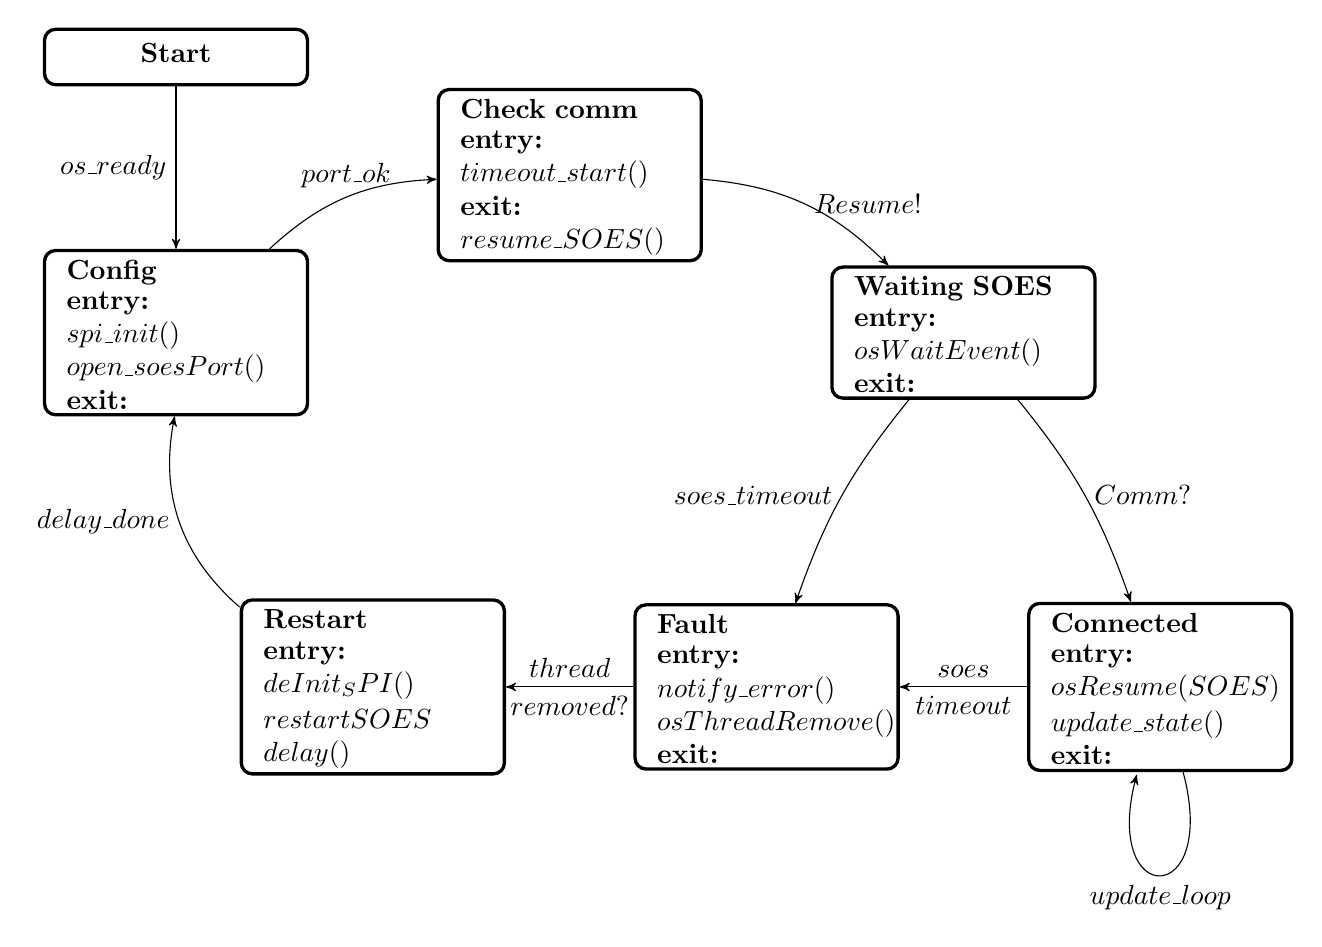
\begin{tikzpicture}[->,>=stealth']
      % Position of QUERY 
      % Use previously defined 'state' as layout (see above)
      % use tabular for content to get columns/rows
      % parbox to limit width of the listing
      \node[state,
          text width=3.2cm 	
          ] (E_CONFIG) 
      {\begin{tabular}{l}
          \textbf{Config}\\[.1em]
          \parbox{4cm}{
          \textbf{entry:}\\
          $spi\_init()$\\
          $open\_soesPort()$\\
          \textbf{exit:}
          }
      \end{tabular}};

      % STATE START 
      % Use previously defined 'state' as layout (see above)
      % use tabular for content to get columns/rows
      % parbox to limit width of the listing
      \node[state,
          text width=3.2cm,
          above of = E_CONFIG,
          node distance = 3.5cm,
          anchor = center] (E_START) 
      {\begin{tabular}{l}
          \textbf{Start}\\[.1em]
          
      \end{tabular}};


          
      % State: ACK with different content
      \node[state,    	% layout (defined above)
          text width=3.2cm, 	% max text width
          yshift=2cm, 		% move 2cm in y
          right of=E_CONFIG, 	% Position is to the right of QUERY
          node distance=5cm, 	% distance to QUERY
          anchor=center] (E_CHCK) 	% posistion relative to the center of the 'box'
      {%
      \begin{tabular}{l} 	% content
          \textbf{Check comm}\\[.1em]
          \parbox{2.8cm}{
              \textbf{entry:}\\
              $timeout\_start()$
              \textbf{exit:}\\
              $resume\_SOES()$
              }
      \end{tabular}
      };
      
      % STATE E_WAIT
      \node[state,
      text width=3.2cm,
          %below of=ACK,
          right of=E_CHCK,
          yshift=-2cm,
          node distance=5cm, 
          anchor=center ] (E_WAIT) 
      {%
      \begin{tabular}{l}
          \textbf{Waiting SOES}\\[.1em]
          \parbox{2.8cm}{
              \textbf{entry:}\\
              $osWaitEvent()$\\
              \textbf{exit:}
              }
      \end{tabular}
      };
      

      
      %STATE CONNECTED
      \node[state,
      text width = 3.2cm,
      below of=E_WAIT,
      xshift= 2.5cm,
      node distance=4.5cm,
      anchor=center] (E_CONNECTED) 
      {%
      \begin{tabular}{l}
      \textbf{Connected}\\[.1em]
      \parbox{4cm}{
          \textbf{entry:}\\
          $osResume(SOES)$\\[.1em]
          $update\_state()$\\
          \textbf{exit:}
          }
      \end{tabular}
      };

      % STATE E_FAULT
      \node[state,
          text width=3.2cm,
          below of=E_WAIT,
          xshift=-2.5cm,
          node distance=4.5cm,
          anchor=center] (E_FAULT) 
      {%
      \begin{tabular}{l}
      \textbf{Fault}\\[.1em]
      \parbox{4cm}{
          \textbf{entry:}\\
          $notify\_error()$\\
          $osThreadRemove()$\\
          \textbf{exit:}
          }
      \end{tabular}
      };

      %STATE RESTART
      \node[state,
      text width = 3.2cm,
      left of=E_FAULT,
      node distance=5cm,
      %xshift = 2cm,
      anchor=center] (E_RESTART) 
      {%
      \begin{tabular}{l}
      \textbf{Restart}\\[.1em]
      \parbox{4cm}{
          \textbf{entry:}\\
          $deInit_SPI()$\\[.1em]
          $restartSOES$\\
          $delay()$
          }
      \end{tabular}
      };

      % draw the paths and and print some Text below/above the graph
      \path
          (E_START)       edge node[anchor=center,left]{$os\_ready$}  (E_CONFIG) 
          (E_CONFIG) 	    edge[bend left=20]  node[anchor=north,above]{$port\_ok$} (E_CHCK)
          (E_CHCK)     	edge[bend left=20] node[anchor=north,right]{$Resume!$} (E_WAIT)
          (E_WAIT)       	edge[bend left=10]  node[anchor=center,right]{$Comm?$}     (E_CONNECTED)
          (E_WAIT)       	edge[bend right=10] node[anchor=center,left]{$soes\_timeout$}                                         (E_FAULT)
          (E_CONNECTED)   edge            node[anchor=north,above]{$soes$}     
                                          node[anchor=south,below]{$timeout$}(E_FAULT)
          (E_CONNECTED)   edge[loop below]  node[anchor=center,below]{$update\_loop$}                   (E_CONNECTED)
          (E_FAULT)  	    edge            node[anchor=north,above]{$thread$} 
                                          node[anchor=center,below]{$removed?$}   (E_RESTART)
          (E_RESTART)  	edge[bend left=30]  node[anchor=center,left]{$delay\_done$}                                          (E_CONFIG)
          ;

      \end{tikzpicture}
  }}\hfill
  \subfigure[SOES application state machine]{\label{subfig:soes_sm}{
      %SOES state machine 80/100
      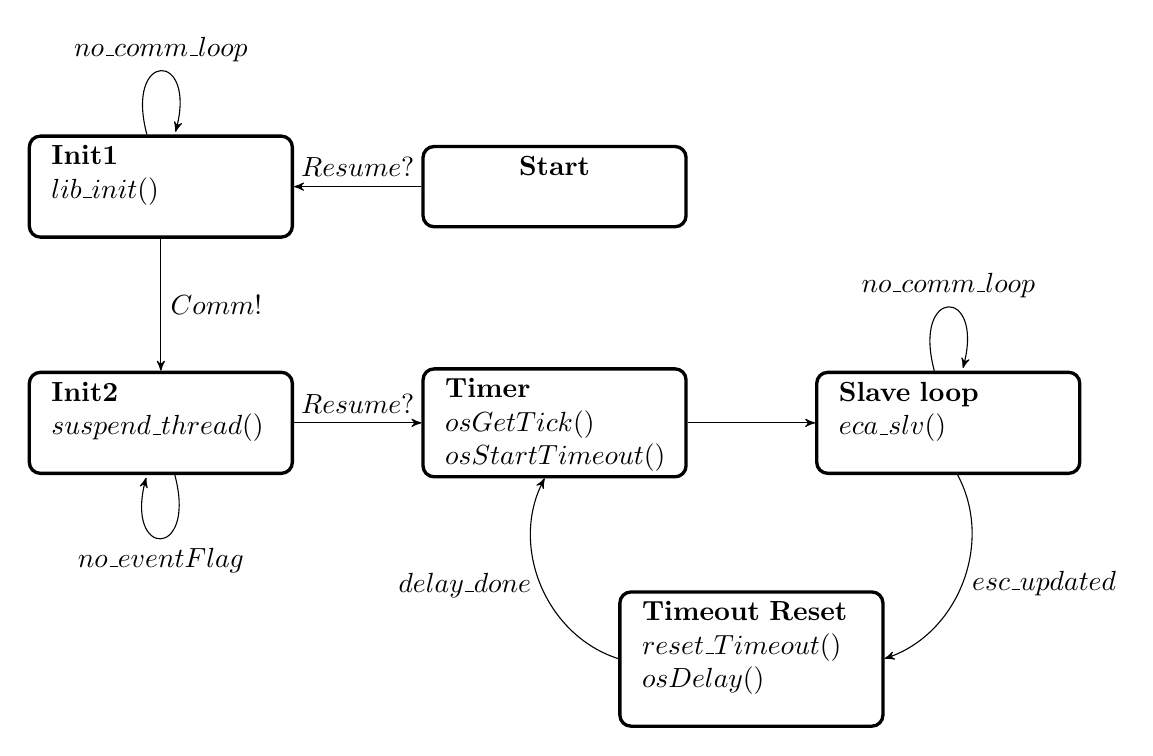
\begin{tikzpicture}[->,>=stealth']
      % STATE 1 SOES
      % Use previously defined 'state' as layout (see above)
      % use tabular for content to get columns/rows
      % parbox to limit width of the listing
      \node[state,
          text width=3.2cm 	
          ] (SOES_INIT1) 
      {\begin{tabular}{l}
          \textbf{Init1}\\[.1em]
          \parbox{4cm}{
          
          $lib\_init()$\\
          
          }
      \end{tabular}};
          
      % STATE SOES INIT 2
      \node[state,    	% layout (defined above)
          text width=3.2cm, 	% max text width
          %yshift=2cm, 		% move 2cm in y
          below of=SOES_INIT1, 	
          node distance=3cm, 	% 
          anchor=center] (SOES_INIT2) 	% posistion relative to the center of the 'box'
      {%
      \begin{tabular}{l} 	% content
          \textbf{Init2}\\[.1em]
          \parbox{2.8cm}{
              $suspend\_thread()$\\
              }
      \end{tabular}
      };

      % STATE 0 SOES
      % Use previously defined 'state' as layout (see above)
      % use tabular for content to get columns/rows
      % parbox to limit width of the listing
      \node[state,
          text width=3.2cm,
          right of = SOES_INIT1,
          node distance = 5cm,
          anchor = center] (SOES_INIT0) 
      {\begin{tabular}{l}
          \textbf{Start}\\[.1em]
          \parbox{4cm}{
          
          }
      \end{tabular}};
      
      % STATE SET TIMER
      \node[state,
      text width=3.2cm,
          %below of=ACK,
          right of=SOES_INIT2,
          %yshift=-2cm,
          node distance=5cm, 
          anchor=center ] (SOES_TIMER) 
      {%
      \begin{tabular}{l}
          \textbf{Timer}\\[.1em]
          \parbox{2.8cm}{
              $osGetTick()$\\
              $osStartTimeout()$
              }
      \end{tabular}
      };
      

      
      %STATE SLAVE LOOP
      \node[state,
      text width = 3.2cm,
      right of=SOES_TIMER,
      %xshift= 2.5cm,
      node distance=5cm,
      anchor=center] (SOES_SLAVE) 
      {%
      \begin{tabular}{l}
      \textbf{Slave loop}\\[.1em]
      \parbox{4cm}{
          $eca\_slv()$\\
          }
      \end{tabular}
      };

      % STATE SOES_RESET TIMEOUT
      \node[state,
          text width=3.2cm,
          below of=SOES_SLAVE,
          xshift=-2.5cm,
          node distance=3cm,
          anchor=center] (SOES_RESET) 
      {%
      \begin{tabular}{l}
      \textbf{Timeout Reset}\\[.1em]
      \parbox{4cm}{
          $reset\_Timeout()$\\
          $osDelay()$\\
          }
      \end{tabular}
      };

      
      draw the paths and and print some Text below/above the graph
      \path
      (SOES_INIT0)    edge node[anchor=center,above]{$Resume?$} (SOES_INIT1) 
      (SOES_INIT1) 	edge  node[anchor=south,right]{$Comm!$}  (SOES_INIT2)
      (SOES_INIT1)    edge [loop above]   node[anchor=east,above]{$no\_comm\_loop$} (SOES_INIT1)
      (SOES_INIT2)    edge [loop below]   node[anchor=south,below]{$no\_eventFlag$} (SOES_INIT2)
      (SOES_INIT2)    edge node [anchor=center,above]{$Resume?$} (SOES_TIMER)                                          (SOES_TIMER)
      (SOES_TIMER)    edge                   (SOES_SLAVE)
      (SOES_SLAVE)    edge [loop above]       node[anchor=center,above]{$no\_comm\_loop$}       (SOES_SLAVE)
      (SOES_SLAVE)    edge [bend left = 50]   node[anchor=center,right]{$esc\_updated$}   (SOES_RESET)
      (SOES_RESET)    edge [bend left = 50]   node[anchor=center,left]{$delay\_done$}   (SOES_TIMER)
      ;

      \end{tikzpicture}
  }}
  \caption{State machines for EtherCAT slave functionality} %EtherCAT Device Protocol poster from EtherCAT resources
  \label{fig:soes_sms}
\end{figure} 

\subsection{Scheduling}
All the SMs and two super states are implemented as Threads using CMSIS-RTOS on STM32. All threads have fixed priorities and the timeslot assigned to each Thread is control by a OS-native delay function, which allows the scheduler to allocate CPU resources to the next priority tasks. The only time constraint is defined as desired so it is no hard real time constraints* and the overall execution follows a best effort approach. This, however, opens the door to further improvement in the sense of characterizing the task durantion. For instance, since it is quite demanding to know the exact precise execution time of each Task and without that is not possible to think about optimizing the OS configuration -if required-, the following is a list of proposed activities that could take place in future stages of the project (out of scope)****. **This is related to a calculation of the Utilization factor that is helpful for more demanding design cases, e.g., while considering heat sinks for processors within enclosed devices.

\begin{description}
\item[Execution Time estimation per task] each task can be isolated by software and through adding a piece of code to toggle a free GPIO at the end of the thread, a signal can be traced with a fair digital analizer (**include example of one ). Omiting the rather small HAL overhead added with the GPIO control, an estimation could be achieved.
\item[Live thread tracing]  a trace debugging like SEGGER SystemView**reference to fastbitlab** can be used to debug freeRTOS applications running on ARM Cortex Mx based Microcontroller such as STM32Fx. With this tool it could be possible to have at runtime a trace of the thread allocations, knowing in consequence the duration of the threads. **Further information regarding this methodology is needed.
\item[Optimization of threads] By knowing the WCET of each thread an optimization of the utilization could be carried out by using differnet OS-native features to improve the scheduling, as long as the application demands it.
\end{description}


**Here comes a table with the priority for each task**

RAte monotonic oder deadline monotonic???


EDF ----Scheduling , is this for dynamic priorities?

\section{PCB}

In this section is described the main stages regarding the manufacturing of the PCB. The schematics and PCB layout can be consulted within the annex X ~\ref{appx:pcb}

\subsection{Development}
\begin{description}
\item[Design] \emph{Altium} PCB design software was used to deliver the \emph{Axis Communication Hub} prototype. During the process the designs from
\item[Manufacturing]
\item[Testing] The overall integrity and functioning of the  Overall power-on and SWD-Programming of the STM32 MCU via SWD/JTAG connector on-board, SPI connections/communication with LAN9252 Evaluation Board. Readout of directly addressed memory space, specificaly test and ID register; PWM Outputs over the two channels for WS2812 LED control, 1 per physical connector and 1-wire connection physycally tested by reading 1-wire sensors, as detailed in ~\ref{sec:temperature}.
\end{description}

**Here comes an image of the PCB mounted on top of the LAN9252 Evaluation Board**


** Question. What would happen if the synchronization mode within an EtherCAT network wants to be integrated to those of a TSN???



\chapter{Results}\label{cha:results}

%Guideline
    % introduction
    % LED PCB and spi captures >> 
    %     challenges only in communication
    %     improvements
    % Scheduling 
    %     TAble with challenges and results
    %     final comments and improvements
    % SOES
    %     Wireshark and twincat screenshots
    %     Challenges breaking the infinite loops and the CPs
        
This chapter starts where the previous chapter left for each of the functional modules, having in mind that the results for the 
temperature are mixed with those of SOES, as the data that is being transferred is now only generated by the sensors. Some photos
and screenshots are presented as well. Challenges, their solving and further improvements are also commented along the chapter.


\section{PCB, SPI and LED control}

In Fig.~\ref{fig:pcb_final} the final PCB prototype can be seen. It is worth mentioning that one issue
emerged
related to the physical requirements of the temperature sensors. 
According to the library integration process commented in Sect.~\ref{sec:temperature}, 
during the first month a rather simplistic approach was coded to have access to the temperature values, the sensors in this approach
used an 
external power source. In contrast, the final sensors were cabled in such a way that they rely on parasite-powered circuitry.
Additionally, the final library that was included made use of the UART peripheral in a full duplex mode, which means that two independent 
pins were explicitly needed, namely RX and TX. That also differed from the first approach's configuration mode. Given this differences, 
only one available GPIO pin with no extra pull-up transistor in the PCB side, was not appropriate to test correctly the 
new one-wire setup. Nonetheless, arrangements were carried out to use the UART RX/TX pins available in the JTAG connector and add external resistors. 
This approach was merely for testing and will be corrected in any further development out of the scope of this Research Project.

\begin{figure}
  \centering
  \subfigure[PCB unmounted]{\label{subfig:pcb_final1}{\includegraphics[width=0.42\textwidth]{imgs/res-pcb01.jpg}}}\hfill
  \subfigure[PCB mounted]{\label{subfig:pcb_final2}{\includegraphics[width=0.42\textwidth]{imgs/res-pcb02.jpg}}}
  \caption{Manufactured PCB.}
  \label{fig:pcb_final}
\end{figure}

The Process Data Interface (PDI) took into consideration the minimal data rate 
calculated for unsigned integers of 16-bit long that would be interpreted
by the Master. This information is summarized in Table~\ref{tbl:minimal_speed}. 

\begin{tuhhtable}
  \begin{tabular}[tp]{L{.18\textwidth}C{.35\textwidth}C{.3\textwidth}}
    \THc{1}{c}{Data} &  \THc{1}{c}{Considerations}&  \THc{1}{c}{Size} \\
    \abovebodyrule
      Temperature       & 15 sensors   &  \SI{30}{\byte}     \\\TRc
      System     & Status, events, errors and parameters data chunk    & \SI{8}{\byte}     \\
      Master               & Commands data chunk& \SI{8}{\byte}     \\\TRc
      IMU            & Acceleration, Magnetometer and Gyroscope for 3 Axis & \SI{36}{\byte}    \\
      BISS-C                 & Data chunk      & \SI{12}{\byte}    \\
    \belowbodyrule
    Total                 &       & \SI{94}{\byte} $\sim$ \SI{128}{\byte}    \\\TRc
    Data rate @ \SI{10}{\milli\second}                 &       & \SI{12.8}{\kilo\byte\per\second}$=$\SI{0.1}{\mega\bit\per\second}   \\
  \end{tabular}
  \caption{Data chunks considered for calculating a minimal data rate at the required refresh rate of the device. }
  \label{tbl:minimal_speed}
\end{tuhhtable}

Another issue that is good to remark, is the noisy communication that emerged at SPI higher speeds. Generally, the monitoring of SPI
signals was very frequently, since the possibility of a fault increased after any new modification, and those needed to be 
traced back to their origin, being sometimes the Host MCU or the LAN9252 chip. Nevertheless, hooking up to the SPI bus introduced another
fault source that was not identified until the communication speeds and their quality were generally characterized. This is, if the GPIOs were 
adjusted to be visualized through a logic analyzer or oscilloscope the communication with LAN9252 was not possible. Hence, 
in order to keep a reliable test environment, it was decided to decrease the SPI data rate without affecting the minimal 
settings 
previously mentioned in Table~\ref{tbl:minimal_speed}. Note that that higher data rate configuration does not imply higher data transmission, as 
the library introduces an almost constant software delay due to the processing of the stack functions, 
namely between \SIrange{2.7}{2.9}{\micro\second}; which starts to be significant as the interface speed goes up. 
The observations regarding this issue are presented in Table~\ref{tbl:spi_speeds}, where symbols imply how good or bad was the communication
between the MCU host and LAN9252, and the visibility through an oscilloscope or digital analyzer. As to the noisy channels at 
high speeds, two screenshots can be seen in Fig.~\ref{fig:signal_noisy}. 

This overall signal integrity problem is rather common within hardware design, therefore, longer times are needed to 
fulfill the requirements
of an optimized hardware when it comes to sensitive data signals. The mentioned working line itself is very broad and 
an introduction for how grounding affects the signal integrity can be consulted in ~\cite{pcb_design_grounding}.%add the reference of pcb desginf for high frequency


%Configuration  GPIO characteristic Speed   LAN9252 stability Logic analizer 
\begin{tuhhtable}
    \begin{tabular}[tp]{C{.14\textwidth}L{.23\textwidth}C{.23\textwidth}C{.23\textwidth}}
      \THc{1}{c}{Config} &  \THc{1}{c}{GPIO setup}& \THc{1}{c}{LAN9252 comm}& \THc{1}{c}{Visibility} \\
      \abovebodyrule
        1       & PU: SS\newline NPU/NPD:\newline SCK/MOSI/MISO   & @\SI{10}{\mega\bit\per\second} \tblBad  & \tblGood     \\\TRc
        2       & PU: SS\newline NPU/NPD:\newline SCK/MOSI/MISO   & @\SI{20}{\mega\bit\per\second} \tblBad  & \tblFair\\
        3       & PU: SS\newline NPU/NPD:\newline SCK/MOSI/MISO   & @\SI{40}{\mega\bit\per\second} \tblBad  & \tblBad  \\\TRc
        4       & NPU/NPD:\newline SCK/SS/MOSI/MISO        & @\SI{2.5}{\mega\bit\per\second} \tblGood  & \tblFair  \\\
        5       & NPU/NPD:\newline SCK/SS/MOSI/MISO        & @\SI{20}{\mega\bit\per\second} \tblFair  & \tblBad  \\\TRc
        6       & NPU/NPD:\newline SCK/SS/MOSI/MISO        & @\SI{40}{\mega\bit\per\second} \tblFair  & \tblBad  \\
        Current         & NPU/NPD: \newline SCK/SS/MOSI/MISO       & \SI{10}{\mega\bit\per\second} \tblGood  & \tblBad  \\\TRc
      \belowbodyrule
    \end{tabular}
    \caption{SPI GPIO configurations affected the communication performance with LAN9252. PU stands for pull-up, whereas NPD, no pull-up nor pull-down. }
    \label{tbl:spi_speeds}
\end{tuhhtable}

\begin{figure}[tp]
    \centering
    \subfigure[Non Pulled-up signal]{\label{subfig:signal_weak}{\includegraphics[width=\textwidth]{imgs/result-signalweak.png}}} \\
    \subfigure[Spikes at higher data rates]{\label{subfig:signal_noisy}{\includegraphics[width=\textwidth]{imgs/result-signalnoisy.png}}}
    \caption{Issues with SPI bus. In ~\ref{subfig:signal_weak} the green signal corresponds to SS pin and demands a pull-up resistor to proper visualization, while LAN9252 demands open-drain pin for correct communication.
            Whereas in ~\ref{subfig:signal_noisy} channels \numlist{1;2;3} show spikes that emerged frequently at speeds higher than \SI{5}{\mega\bit\per\second}, leading to an incorrect recognition of the clock (CLK) signal.}
    \label{fig:signal_noisy}
\end{figure}


With reference to the LED results, besides the challenge that personally represented the library adaptation and the usage of the DMA 
peripheral, the functionality was stable.

An open point which did not represent an obstacle for the project, but keeps the door open for further improvement is 
the possibility of using more than one channel per PWM generator. The reason why this was not implemented lies with 
the time required for testing. The straightforward option is to use one DMA channel and one PWM Channel per ring, 
for the MCU host contains two DMA peripherals, each with 8 streams and each stream in turn with 8 channels---technical
specifications can be seen in ~\cite{stm32f446_data}; 
therefore, it did not represent any problem. 
Nonetheless, it could be argued that only one PWM generator could control up to four Led Rings, as long as each PWM channel is updated through
an individual DMA channel, this way the hardware would be used more efficiently. The MCU should only have ready each memory buffer 
to start the transmission of the serial data. This approach would apparently imply larger space, but if the color data 
is taken 
out from an unique buffer that is updated on-the-fly for the next LED interface, the efficiency, at least regarding usage of HW, will be better. 
Consequently, this could also lead to use two DMA streams at the same time for a total of eight rings with only two PWM generators 
and two DMA streams. 

Anyhow, the before mentioned approach needs expertise with DMA peripheral and formal evaluation of the benchmarks related to 
the utilization
of the processor and memory footprint moreover, the optimization of this LED control is not part of the scope of this project, and 
better use of this peripheral is apparently exploited in other applications such as graphics rendering---see application in ~\cite{stm32_dmaapp}---or 
transferring of
memory chunks at way faster speeds. The latter could be though interesting, since the LAN9252 counts with a Quad-SPI interface.
%https://auto.siili.com/blog/optimizing-rendering-performance-on-stm32-using-dma2d
%Add reference to the Direct memory access DMA




\section{DSMs and RTOS integration}\label{sec:scheduling_results}

%Guidelines
% introduction
% --------------------
%     Mention the scheduling apporach of RTOS
        
%         List of proposed threads and description of them (only proposal)
%         Priority based, fixed and not based on Execution times
%            >> Time proposed for each one, mention that it is also configurable. 
%           SPI speed calculation?
%         This is a Table
     
% ---------------------This is in results-----------------------------------
%     Problems in the implementation 
%         Priority of each task + timer priority
%             Solutions + Task manager
%          Present the final table of threads
%         explains events its problems with timers, etc    
%             Solutions
%     List of resources that might demand mutex
%             List of general variables
%         Regardinf the synchronization: How the OS prevents from problems?
%             solutions
%           Future improvement (3 items for OS debugging)

As introduced during the implementation description, Sect.~\ref{sec:scheduling_intro}, this part will comment a bit further the results
of the usage of FreeRTOS to schedule and synchronize the execution of the DSMs, such that a deterministic behavior 
could be reached. Similar to the previous section, some issues and comments about it are presented along the
way.
\subsection{Final scheduling and synchronization}
To start with, in the Table~\ref{tbl:threads_final} the current list of threads can be seen. Important to point out is the necessity 
to define carefully priorities besides the previously given \emph{desired} release times. In the same table an 
OS-defined thread is included that was crucial for the current SW structure, namely \emph{osTimer Daemon Task}. 

\begin{tuhhtable}
    \begin{tabular}[hb]{L{.3\textwidth}C{.3\textwidth}C{.3\textwidth}}
      \THc{1}{c}{Thread} &  \THc{1}{c}{Priority}&  \THc{1}{c}{Release period} \\
      \abovebodyrule
        User Task Manager       & osPriorityHigh    & Event driven     \\\TRc
        osTimer Daemon Task     & osPriorityHigh    & Event driven     \\
        Event Handler SDM               & osPriorityAboveNormal& Event driven     \\\TRc
        SOES APP SDM            & osPriorityAboveNormal& \SIrange{5}{10}{\milli\second}     \\
        LED SDM                 & osPriorityNormal      & \SI{33}{\milli\second}    \\\TRc
        ECAT SDM*               & osPriorityNormal      & \SI{100}{\milli\second}     \\
        Temperature SDM         & osPriorityNormal      & \SI{1000}{\milli\second}     \\\TRc
      \belowbodyrule
    \end{tabular}
    \caption{Final priorities' arrangement for main threads. \emph{*ECAT SDM 
        is mainly event driven, nevertheless, in the connected state it has a periodic update}}
    \label{tbl:threads_final}
\end{tuhhtable}

Regarding the \emph{User Task Manager}, its implementation was meaningful because of the suspension/termination of threads was taken place
within the synchronization of ECAT and SOES DSMs---recall the synchronization signals in the DSM in Sect.~\ref{sec:statemachines}. 
For instance, due to the way the library is coded, every time there is a communication breakdown, SOES goes into an infinite loop 
as it is polling continuously ESC state registers instead of using and IRQ pin---review SM-Synchronous in Appendix~\ref{sec:synch_managers}---. 
Other sources of this infinite loops that demands forcing a thread to stop are the physical connection problems, such as the ESC power-off, 
cable disconnection, power source drop, etc. 
Given these scenarios, clearly a solution with timeout control was tried out but the low level timers (HW peripherals) induced problems
as it is of high caution mixing hardware interrupts when running an OS.
Therefore, the Task Management events are sent with help of callback functions from osTimers (Timers implemented by the OS). 
As to the latter, they are really managed by the so-called osTimer Daemon Task and are fully configurable. However, a few characteristics need to be taken 
into account as the Daemon runs as hidden Task for the user, in addition, if this Task is not correctly set the callbacks can be lost 
as the Damon tries to interrupt a higher priority task. Some parameters to configure are callback stack depth, queue length and priority. 
More information regarding this topic can be found in \emph{Timer Management} section of ~\cite{cmsis_doc}.

Coming back to the infinite loop issue, once the timers are set and can correctly interrupt, if one task is within an infinite loop, keeping its own 
state machine from continue and consequently others, then a fault is emerged. Then the osTimer creates an event and suspend or restart the faulty threads.
However, this is actually something that the Event Handler should take care of, or any other thread, since the OS-defined functions
related to thread management cannot be executed from ISR ---not even software interruptions. Furthermore, the suspension or termination of
threads need to be handled with care, since if a thread is suspended or terminated right after a higher priority task preempts the callback
function---imagine the Event Handler SDM being of higher priority than SOES App SDM---as soon as the higher priority task finishes, the callback 
function would be executed but as the OS would try to
go back to the thread where it was originally called, and this has been put out of the execution queue, it would result in an OS hard fault.

Therefore, using a simple user-defined Task Manager thread that is constantly waiting for event flags or periodically updating their states, 
makes possible to manipulate threads, and therefore it has been the current solution to avoid some problems. However, 
less complicated approaches are being taken
into account for further generalization, since deleting and creating tasks might have stability problems regarding the fragmentation
of the heap. Sometimes, hard faults may appear and would be very hard to identify which memory overflow might have caused it.

Just as the previous example, hard faults---not surprisingly---are to be avoided, but doing this efficiently demands rather \emph{good strategy}.
What is more, this situation could repeat in other conditions, even due to implementation of the OS. For example, there are even 
OS-functions that are explicitly described as being compatible with execution from ISRs, though they might have no effect, as it was the 
case for Event Flags---even ensuring
their respective volatile definitions; or in the case of waiting states within a DSM. The last-mentioned can also lead to hard fault, 
since the execution of an unique Task 
that ends up calling apparently endless osDelay functions is considered as faulty condition by the OS.

\begin{tuhhtable}
  \begin{tabular}[ht]{L{.25\textwidth}L{.5\textwidth}}
    \THc{1}{c}{DSM Event} &  \THc{1}{c}{Main use} \\
    \abovebodyrule
      SYS\_EVENT    & Events and errors sent to the Event Handler DSM\\\TRc
      LED\_EVENT    & Internal LED DSM events\\
      TSENS\_EVENT  & Internal Temperature DSM events\\\TRc
      ECAT\_EVENT   &  Synchronization between ECAT DSM and SOES APP\\
      TASKM\_EVENT  & Thread management/update request from any DSM\\\TRc
    \belowbodyrule
  \end{tabular}
  \caption{Events between DSMs are implemented over \emph{Event Flag Signals} managed by the OS.}
  \label{tbl:events_sms}
\end{tuhhtable}

In relation to the mentioned synchronization events, the \emph{OS Event Flags Signals} feature was used. This is basically 32-bit long 
data shared between threads and managed by the OS, that can be related to suspension and resume of threads according to the bits (flags)
that are set or clear with \emph{OS Wait} functions. Some details could be not as clear as they should be, since working conditions
vary among OS layers, this is for example, the FreeRTOS defines the signals as 32-bit unsigned integer with the 31st bit reserved for internal
error flag; nonetheless, on top of it the CMSIS v2 defines in turn the same signal as the same integer but only 24 bits available. 
If 
the application works with any flag bit between the 24th and the 30th bit, the final OS layer returns no error but does not notify any
thread. A list of the main signals used for synchronization between DSM is presented in Table~\ref{tbl:events_sms}, whereas a list of the events
and errors so far implemented in the Event Handler DSM's logic is showed in Table~\ref{tbl:events_errors}. However, a complete list of events and
errors can be seen in the header code within Appendix~\ref{appx:code}.

\begin{tuhhtable}
  \begin{tabular}[bp]{L{.3\textwidth}L{.4\textwidth}}
    \THc{1}{c}{ACB Event} &  \THc{1}{c}{ACB Error} \\
    \abovebodyrule
      EV\_TEMP\_DSM\_INIT       &  ERR\_TEMP\_DSM\_FAULT     \\\TRc
      EV\_LED\_DSM\_INIT     &   ERR\_TEMP\_SENS\_OVERHEAT   \\
      EV\_ECAT\_DSM\_INIT               &ERR\_TEMP\_SENS\_LOST*  \\\TRc
      EV\_ECAT\_CMD\_ACK            &ERR\_LED\_DSM\_FAULT \\
      EV\_ECAT\_APP\_OP                 &   ERR\_ECAT\_DSM\_FAULT    \\\TRc
      EV\_ECAT\_APP\_INIT              & ERR\_ECAT\_CMD\_FAULT*      \\
      EV\_ECAT\_CMD\_ACK         & ERR\_ECAT\_CMD\_SOFTFAULT*      \\\TRc
        &ERR\_ECAT\_COMM\_LOST\\
        &ERR\_SYS\_UNKNOWN\\\TRc
    \belowbodyrule
  \end{tabular}
  \caption{DSM's events and errors considered by Event Handler DSM. \emph{*Currently being implemented.}}
  \label{tbl:events_errors}
\end{tuhhtable}

\subsection{Further development}
Finally, there are two topics open for future, first one has to do with shared memory, while the second is about optimization of the
scheduling approach. Regarding the former, so far no complication has appeared in the rather non-critical data being transmitted, namely
the buffer that both the Temperature and the SOES App update. Currently, an approach an easy approach that can be implemented is using
again the events to notify the SOES APP whenever the Temperature App has updated its buffer. Other is using the MUTEX feature implemented
in the OS. Both approaches are planned. Going back to the mentioned topics, the latter could be at this stage difficult, as it needs
the precise execution time of each Task to be known. Without it is not possible 
to think about optimizing the utilization or the OS configuration in a more detailed manner -if even required-. 
For instance, in the future calculation 
of the \emph{Utilization} factor will be helpful for optimizing scheduling, but it could be also needed in more practical design cases, 
e.g., 
while considering heat sinks for processors within enclosed devices. Therefore, the following is a list of proposed 
activities that could take place in future stages out of scope of the current Research Project. 

\begin{description}
\item[Execution Time estimation per task] Each task can be isolated by software. Then, by adding a piece of code to toggle a free GPIO 
      at the end of the thread, a signal can be traced with a fair digital analyzer. Omitting the rather small HAL 
      overhead added with the GPIO control, an estimation of the execution time can be achieved.
\item[Live thread tracing]  A trace debugging like SEGGER SystemView, see ~\cite{rtos_segger},%**reference to fastbitlab** 
    can be used to debug freeRTOS applications running on ARM Cortex Mx based Microcontroller such as STM32Fx. 
    With this tool it could be possible to have at runtime a trace of the thread allocations, knowing in consequence the duration 
    of the threads. 
\item[Optimization of threads] By knowing the Worst Case Execution Time (WCET) of each thread an optimization of the utilization could be carried out 
    by using different OS-native features to improve the scheduling, as long as the application demands it.
\end{description}

\section{SOES library integration}

The results presented in this section implies the correct functionality of the temperature functional block.
% Understand the variations between Little/Big Endian within buses. That the library is based on polling by one by one the unique FIFO register of the ESC, such that the PDOs can be written and read in the PD RAM, as it was thought that a direct access to the RAM would permit the User Address Space of the MCU to be extended and the access then would be transparent for manipulating the data,  and that the SM would permit only the safe access from the Master device to read/write the same address space. It could be then understood that there is a significant delay that van be even measure, that in some papers is determined as "Stack Delay" which in this case *Reference the paper of the design of the communication/delay analysis*.
% The advantages of reducing it through the implementation of the SQI or the HSI interface -which at the end does not have that much purpose since for achieving less delays the FPGA or ASIC maybe implemented-. The question, is it still sensible to develop EtherCAT devices with this approach or should it be switched completely to the FPGA and ASIC approach. An analysis considering costs and other things could be then carried out. ***
% **Making available the Szstem Interrupt Controller without polling would also increase the performance of the application, this can be aimed in next versions where physically the the pins are connected to the Host MCU.
% **A brief analysis of the bandwidht achieved as the bandwidth necessarz to make sensible a change of PDI would make sensce, since the HBI****reference to internet or anz specification of HBI*** is mainly foucsed to Board-To-Board connections or communication between ASICS, hence  4Gbps per pin die-to-die connectivity with low latency may not be needed at all *https://www.synopsys.com/designware-ip/interface-ip/die-to-die.html**.
% **Important to mention is the HBI only helps exchanging process data, so it could be implemented for applications where data chunks are needed to be transmitted at high bandwidth since it is a direct fifo access to the ESC's SRAM.
% **Here should be also commented the problems by reading and writing, mainly writting due to the noisy medium (cabling).
In the Fig.~\ref{fig:ecat_wireshark} the transition from safe-operation (SAFEOP) to operation state (OP) of the EtherCAT device is shown. 
The operation state can only be reached when the Object Dictionary has been correctly matched between the Master and the device
through the SMs, a synchronization mode has been correctly configured and the AL registers can be correctly read and written 
by both devices. The protocol makes use of DLL commands to broadcast state change requests to the slaves, afterwards it broadcasts 
a read command. Each device connected will react and update its corresponding AL state register. 

\begin{figure}[h]
  \centering
  \includegraphics[width=\textwidth]{imgs/result-wireshark-preop-op1.JPG}
  \caption{Transaction of data frames between Master and Slave during a state change request.}
  \label{fig:ecat_wireshark}
\end{figure}

In addition, it is important to 
recall that the working counter at the end of the data structure that points out whether a device in the network has processed 
the data frame or not, review the frame structure in Appendix~\ref{sec:ecat_protocol}. Having the frame in mind, it is possible to 
recognize all its parts, as the the communication trace was monitored with Wireshark. Hence the detailed interaction between parties 
through the updated data frames is clearly seen in Fig.~\ref{fig:ecat_wireshark2}.


\begin{figure}[ht]
  \centering
  \subfigure[BRD command to read current AL state register]{\label{subfig:cmd1}{\includegraphics[width=0.7\textwidth]{imgs/result-wireshark-preop-op2.JPG}}}\\
  \subfigure[FPWR command to write a request to AL control register]{\label{subfig:cmd2}{\includegraphics[width=0.7\textwidth]{imgs/result-wireshark-preop-op3.JPG}}}\\
  \subfigure[BRD command to read current AL state register]{\label{subfig:cmd3}{\includegraphics[width=0.7\textwidth]{imgs/result-wireshark-preop-op4.JPG}}}
  \caption{Detailed request and response for a state change. SAFEOP to OP state is the last change starting from INIT state.} %EtherCAT Device Protocol poster from EtherCAT resources
  \label{fig:ecat_wireshark2}
\end{figure}

Finally, in Fig.~\ref{fig:ecat_twincat_objects} the input and outputs part of the object dictionary is shown after it can be 
accessed through TwinCAT3. A whole definition of it is though included in the Appendix~\ref{app:esi_file}.

\begin{figure}[hb]
  \centering
  \subfigure[Process data input]{\label{subfig:objectdictionary1}{\includegraphics[width=0.68\textwidth]{imgs/result-objectdictionary2.png}}}\\
  \subfigure[Process data output]{\label{subfig:objectdictionary2}{\includegraphics[width=0.68\textwidth]{imgs/result-objectdictionary3.png}}}
  \caption{Object Dictionary from TwinCAT interface.} %EtherCAT Device Protocol poster from EtherCAT resources
  \label{fig:ecat_twincat_objects}
\end{figure} 

% \subsubsection{SPI communication}
% **This is a draft, this might not be needed
% During the final tests some communication errors appeared that were tracked back to the following conditions: %TODO Investigate if this can be called failure modes
% \begin{description}
%     \item[Voltage drops] The on-board Low-Dropout voltage regulator* LDO that provided 3.3 V had random failures, where 
%     the output voltage was from 3.28 to 3.29 V. This caused that the LAN9252 chip was not always ready to work as intended. 
%     This behaviour increased from not-happening to failed completely to start. The mentioned condition obly affected the ESC functionalities,
%     whereas the host MCU worked realiably. To revert this failure mode, an external 3.3V power source was used to continue
%     the current tests. 
%     \item[Noisy channels] While troubleshooting the communication problems mentioned above, an SPI communication
%     test was carried out, such that the effects of different configurations could be characterized. It was concluded that
%     the higher frequencies the SPI was set up, the greater communication faults appeared, leading to error states in the 
%     internal SMs. Moreover, even within rhe stable range, the higher frequencies were not implying shorter execution times.
%     A summary of this observations are presented in the table ~\ref{dummy}.  
% \end{description}
% Regarding the no-improvement of the execution time at a high-speed SPI configuration, the figure ~\ref{dummy} shows 
% a relatevely constant software delay within the words being sent over the SPI bus. Therefore, it does not matter how fast the
% words are sent, for this Software delay is always present *write the order of the delay*. This emergent characteristic of
% the system could be optimized as long as it is determined, whether its impact is critical on the overall throughput of the system.
% The reader should take into consideration the rather small amount of data and the refresh speed of the overall system. However, this
% could be a stating point for improvement of the SOES stack, for those SW delays can be approached by using a fixed sending buffer
% through DMA instead of the usage of the native* API functions that send word by word. A further evaluation of the worthiness*
% of the library changes may be needed.*
% The above mentioned challanges are addressed within the proposals for improvement presented in the section ~\ref{sec:improve}.





\chapter{Conclusions and further development}\label{cha:conclusions}

Overall status: Board and basic SOES features ready for further EtherCAT development.

Even though, there have been delays due to the libraries being ported, and channels being noisy before having the PCB working, we're in a stage where we can ensure that the PCB manufactured and ported libraries allow to further develop an EtherCAT compatible application. Therefore, in the following calendar days the following tasks will be priorized to complete the main tasks:

\section{Further development}\label{sec:improve}

**Inserts probably the challenges in the same strutcture as in the implementation part.



% Bibliography
% if you have cited papers that are not referenced, but important for your work,
% uncommented the following line; however, this should generally by unnecessary
% and hints at improper citing.
% \nocite{*}

\tuhhbibliography{thesis}


% Appendix
% Feel free to add additional appendix chapters (e.g., measurement setups, etc.)
%Code should be added as an appendix?
\begin{tuhhappendix}
  \chapter{Introduction to the EherCAT protocol}\label{sec:ecat_protocol}

As mentioned in the introduction, EtherCAT is an industrial Communication Profile developed by Beckhoff that is 
standardized in the IEC 61588 under the RTE CPF. The development within this company is oriented to the use of 
open standards to increase its impact within the industry, but not only reduced to it but the overall field of smart cities[?], in
a certain degree this approach eliminates the need for many expensive "black boxes"\cite{beckhoff_automation}. %%Beckhoff_Urban_Automation_2013_e almost the introduction thing 
This implies that the interoperability of devices is almost guaranteed, at least from the specification perspective,
not only for private development centers but also for any other developer that follow the standards; if the standards 
are of public access, then this is a mean of empowerment of any group that might be willing
to create its own industrial-compatible technologies.

The OSADL emphatized in 2008 \cite{beckhoff_vs_osadl}, for example, a vision for leading the integration
of opensource in the industry by using the Linux Kernel as a certified Industrial RT (IRT) operative system for industrial embedded applications. 
Back in that day, Beckhoff was involved in that discussion representing the contrary model. Nonetheless, in the last months the same company has
apparently retaken the opensource iniciative by the introduction of the FreeBSD compatible version of the TwinCAT Runtime\cite{beckhoff_freebsd}.%https://www.heise.de/newsticker/meldung/Open-Source-trifft-die-Industrie-201855.html
%**https://www.beckhoff.com/english.asp?highlights/twincat-bsd/default.htm

In comparison with other RTE profiles, EtherCAT has shown a higher performance, more flexible topology and lower costs than other ethernet fieldbus 
technologies. This  protocol  applies  a  master-slave  mode,  in  which  the  master  
device  uses  standerd  100BASE-TX  ethernet  adapter  and  the  ESC  (EtherCAT  Slave  Controler), that implements a EtherCAT IP 
(intellectual property) core within an ASIC or a FPGAto process the frames. As  the  working  cycle starts, the  EtherCAT master  
publishes a frame encapsulated a standardized 8802.3 frame. When the it reaches an ESC, it analyses the address and location on the frame, decides
which parts of it are useful sections and then reads or writes data on it. As the
read-write operation finishes, the Working Counter (WKC) at the end of the frame is added by one, this way the data on the frame has been processed. 
This cycle repeats for each ESC within the topology.%Motion Control System using SERCOS over EtherCAT
EtherCAT supports almost all kinds of topology structure, such as ring, line, star and tree. The transmission speed of  EtherCAT  is  fixed  to  100  
Mbit/s  with  full  duplex  communication.  The  EtherCAT  network  is  able  to  connect  maximally 65535  devices  via  switch  and  media  converter.  
The  EtherCAT  system  can  update  1000  I/Os  in  just  30  microseconds  or  exchange  1486  byte  contents  in  300  microsecond. \cite{beckhoff_datasheet}\cite{ecat_sercos}  %Motion Control System using SERCOS over EtherCAT

Important to highlight is that other CPs are also integrated as services inside the protocol, as previously mentioned for 
the SERCOS specification in \ref{sec:applications}. 
Other examples of these integrated CPs are File over EtherCAT (FoE) or Ethernet over EtherCAT (EoE), which
make possible to support a wide variety of devices and application layers in the same network\cite{beckhoff_compatibility}. %https://www.ethercat.org/en/technology.html#1.9
A complete list of the communication profiles that are on hand
through the protocol's mailboxing is given below, as to the overall layered integration can be seen in figure \ref{fig:ecatprofiles}.
\begin{itemize}
    \item CoE: CAN application protocol over EtherCAT
    \item SoE: Servo drive profile, according to IEC 61800-7-204 (SERCOS protocol)
    \item EoE: Ethernet over EtherCAT
    \item FoE: File Access over EtherCAT (HTTP,FTP,etc)
    \item AoE: Automation Device Protocol over EtherCAT (ADS over EtherCAT)
\end{itemize}

\begin{figure}[ht]
    \centering
    \includegraphics[width=.65\textwidth]{imgs/intro-ecatprofiles.jpg}
    \caption{Different communication profiles can coexist in the same system.}
    \label{fig:ecatprofiles}
\end{figure}

An EtherCAT device with switchport properties usinge EoE would be the equivalent of the TSN compliant
switches, since they would insert any non time-senstitive TCP/IP fragment into the EtherCAT traffic preventing
in this way the real time properties from being affected. Furthermore, the architecture of the protocol itself and
its early cooperation with the IEEE 802.1 group and the OPC Group ensure its continuos compatibility with the
standardization of TSN, OPC UA and the IoT paradigm.\cite{beckhoff_compatibility}%https://www.ethercat.org/en/technology.html#1.12

A slave device must comply at least with CoE and the Mailbox, whereas the Master may comply with all the communication profiles. This of course
needs to be suited to the requirements of the application and the degree of tlexibility that is to be achieved. Consequent certification process
should adhere to Beckhoff's specifications.\cite{beckhoff_slavetutorial} %<< Add the reference to the implementation guide of beckhoff

Having presented this brief summary of the EtherCAT technology, the reader may continue to the implementation chapters. 
More detailed information of the protocol itself that was needed to understand the function of the SOES library
can be read in the section \ref{sec:soes}.


% *Add the image of the Ethernet frame having the EtherCAT datagram inside.
% *Explain the XAE tool and the PDI meaning
% *Quote maybe from paper section BASICS OF ETHERCAT AND PROFINET IRT Network Delay Analysis of EtherCAT and PROFINET IRT Protocols***
%** Question. What would happen if the synchronization mode within an EtherCAT network wants to be integrated to those of a TSN???


\begin{figure}[ht]
    \centering
    \includegraphics[width=\textwidth]{imgs/impl-dataframe.jpg}
    \caption{EtherCAT Datagram within the Ethernet Frame. Source: ETG.1000.4 - EtherCAT frame structure.}
    \label{fig:dataframe}
\end{figure}

\subsubsection{The data frame and the Synchronization Managers}\label{sec:synch_managers}
*Redaction style at 85/100

Besides the challange of setting up the hardware and basic firmware for a correct data transmission between ESC and the host MCU; the description of the EtherCAT 
Slave device is a task that demands, at least, a basic understanding of the data frame exchange and how the protocol demands its synchronization. From here on, the following
topics are going to be summarized: Synchronization modes and managers.
Whenever there are Real Time constraints, and the device takes part of a control loop, synchronization modes are needed to be set correctly between the Master and
any Device present. For this task the Distributed Clocs (DC) are need to be synchronzied. [?][?] %ETG.1020 - Synchronization and ETG.2000 - DC

There are three synchronization modes:  
\begin{description}
    \item[Free Run] Application is triggered by local clock and runs independently of EtherCAT cycle. 
    \item[SM-Synchronous] Application is synchronized whenever there are process data being written to the Synchronization Manager 2 (SM2).
    Moreover, any event generated by the Master is mapped onto an internal register or physically triggering an IRQ Pin of the ESC. 
    \item[DC-Synchronous] Within this synchronization mode the frame jitter can be even reduce down to $ns$ and use two different synchronization
    units within the ESC, namely the SM2 and SYNC/LATCH UNIT. 
\end{description}

The scope of this prototype covers the Freerun and SM-Synchronous mode, as they are the basic ones for communication Master-Slave. A graphical representation of them
is shown in figure \ref{fig:syncmodes}.

\begin{figure}[ht]
    \centering
    \subfigure[Free Run]{\label{subfig:syncm1}{\includegraphics[width=0.3\textwidth]{imgs/impl-sync1.jpg}}}\hfill
    \subfigure[SM-Synchronization]{\label{subfig:syncm2}{\includegraphics[width=0.3\textwidth]{imgs/impl-sync2.jpg}}}\hfill
    \subfigure[DC-Synchronization modes]{\label{subfig:syncm3}{\includegraphics[width=0.3\textwidth]{imgs/impl-sync3.jpg}}}
    \caption{Synchronization modes defined in ETG.1000. Source [?]} %EtherCAT Device Protocol poster from EtherCAT resources
    \label{fig:syncmodes}
\end{figure} 

SMXs (Synchronization Managers 1,2,3 ...) coordinate access to the ESC memory from both sides, EtherCAT and
Host MCU (PDI). In case of process data communication it ensures that process data can
always be written to the memory by EtherCAT and can always be read by PDI side and vice versa (3-buffer mode). SyncManager 2/3 length is equal
to the Data Object lengths defined for receive and transmit data chunks respectively. [?] %ETG.1000.4 Sync manager
The mapping of the process data objects within the Ethernet Frame can be seen in figure \ref{fig:dataframe} and \ref{fig:pdomapping}.
The correct setup of the SMXs ensure the consistency of the data and needs to be linked correctly depending on the specifactions of each type of ESC,
 and SW Stack that are being used, this information is also linked to the CoE Object Dictionary (OD) and EtherCAT Slave Information (ESI) file.
\begin{figure}[ht]
    \centering
    \includegraphics[width=.85\textwidth]{imgs/impl-dataframe_pdo.jpg}
    \caption{Depending on the different states of the Slave, there will be different data frames being exchanged with the Master. 
    The above one corresponds to the Proces Data Object which is updated continuosly by the SM2/3 during Operation State. Referece: 
    ETG.1000.6-SDO}
    \label{fig:pdomapping}
\end{figure}
  \chapter{Device State Machines (DSMs)}\label{cha:state_machines}
%LED control
\begin{figure}[h]
    \centering
    \includegraphics[width=\textwidth]{imgs/dsm_led.png}
    \caption{DSM for LED control functionality.}
    \label{fig:dsm_led}
\end{figure}
%event handler
\begin{figure}[h]
    \centering
    \includegraphics[width=\textwidth]{imgs/dsm_event.png}
    \caption{DSM for Event handler functionality.}
    \label{fig:dsm_event}
\end{figure}
%ecat
\begin{figure}[h]
    \centering
    \subfigure[Synchronization state machine.]{\label{subfig:ecat1}{\includegraphics[width=\textwidth]{imgs/dsm_ecat1.png}}}\\
    \subfigure[SOES application state machine.]{\label{subfig:ecat2}{\includegraphics[width=\textwidth]{imgs/dsm_ecat2.png}}}
    \caption{DSM for EtherCAT functionality.}
    \label{fig:dsm_ecat}
\end{figure}
%temperature
\begin{figure}[h]
    \centering
    \subfigure[Synchronization state machine.]{\label{subfig:temp1}{\includegraphics[width=\textwidth]{imgs/dsm_temp.png}}}\\
    \subfigure[One-wire application state machine.]{\label{subfig:temp2}{\includegraphics[width=\textwidth]{imgs/dsm_temp2.png}}}
    \caption{DSM for Temperature functionality.}
    \label{fig:dsm_temp}
\end{figure}
  \chapter{PCB drawings and layout}\label{appx:pcb}

**here comes  the electrical diagrams and the pcb layout exported by Altium**

  \includepdf[pages=-,landscape=true]{imgs/Schematic Prints_color.pdf}
  \chapter{ESI file definition}\label{app:esi_file}
The following code does not include the lines for the object dictionary as those are rather too extensive for the document. 
Nevertheless, the reader is invited to pay attention to the SM descriptors and the EEPROM configuration word that are those that
need to be adjusted accordingly to the used hardware and the Software Stack.
For even more information regarding the XML specifications according to EtherCAT protocol, resource~\cite{beckhoff_esi} can be 
reviewed.
\begin{lstlisting} [label=lst:esi,caption={Part of the EtherCAT Slave Information file.}]
    <?xml version="1.0" encoding="utf-8"?>
    <EtherCATInfo xmlns:xsi="http://www.w3.org/2001/XMLSchema-instance" xsi:noNamespaceSchemaLocation="EtherCATInfo.xsd" Version="1.2">
      <Vendor>
        <Id>#x00485247</Id>
        <Name>Hans Robot Germany GmbH</Name>
        <!--Here comes a 16X14 image of the company-->
      </Vendor>
      <Descriptions>
        <Groups>
          <Group>
            <Type>COMMBOARD</Type>
            <Name>AXIS_COMM</Name>
            <!--Here comes a 16X14 image of the device-->
          </Group>
        </Groups>
        <Devices>
          <Device Physics="YY">
            <Type ProductCode="#x12783456" RevisionNo="#x00000001">axcommb</Type>
            <Name><![CDATA[AxisCommBoard slave]]></Name>
            <Info>
              <StateMachine>
                <Timeout>
                  <PreopTimeout>8000</PreopTimeout>
                  <!--4 Times from original value-->
                  <SafeopOpTimeout>36000</SafeopOpTimeout>
                  <BackToInitTimeout>20000</BackToInitTimeout>
                  <BackToSafeopTimeout>800</BackToSafeopTimeout>
                </Timeout>
              </StateMachine>
              <Mailbox>
                <Timeout>
                  <RequestTimeout>400</RequestTimeout>
                  <!--4 Times from original value-->
                  <ResponseTimeout>8000</ResponseTimeout>
                </Timeout>
              </Mailbox>
            </Info>
            <!-- Added from SSC TOOL-->
            <GroupType>COMMBOARD</GroupType>
            <Profile>
              <ProfileNo>5001</ProfileNo>
              <Dictionary>
                <DataTypes>
                    <!--DataTypes are omitted-->
                </DataTypes>
                <Objects>
                    <!--Objects are omitted-->
                </Objects>
              </Dictionary>
            </Profile>
            <!-- Added from SSC TOOL-->
            <Fmmu>Outputs</Fmmu>
            <Fmmu>Inputs</Fmmu>
            <!--Is this Fmmu needed?-->
            <Fmmu>MBoxState</Fmmu>
            <!-- ADDRESSES to be checked. So far the addresses match with linux_lan9252 example-->
            <Sm ControlByte="#x26" DefaultSize="128" Enable="1" StartAddress="#x1000">MBoxOut</Sm>
            <Sm ControlByte="#x22" DefaultSize="128" Enable="1" StartAddress="#x1080">MBoxIn</Sm>
            <!--SMs addresses adjusted to from SSC file to SOES-->
            <Sm DefaultSize="8" StartAddress="#x1100" ControlByte="#x64" Enable="1">Outputs</Sm>
            <Sm DefaultSize="36" StartAddress="#x1400" ControlByte="#x20" Enable="1">Inputs</Sm>
            <RxPdo Fixed="true" Mandatory="true" Sm="2">
              <Index>#x1600</Index>
              <Name>MasterCMDs process data mapping</Name>
              <!--Entries are omitted-->
            </RxPdo>
            <!-- Added from SSC TOOL-->
            <TxPdo Fixed="true" Mandatory="true" Sm="3">
              <Index>#x1A00</Index>
              <Name>Input mapping 0</Name>
              <!--Entries are omitted-->
            </TxPdo>
            <!-- Added from SSC TOOL-->
            <Mailbox DataLinkLayer="true">
              <!-- From SSC TOOL: PDOAssign false, pdoConfig false, CompleteAccess true,segmentsdo true-->
              <CoE SdoInfo="true" CompleteAccess="false" PdoConfig="false" SegmentedSdo="true" PdoAssign="false" PdoUpload="true"></CoE>
            </Mailbox>
            <Dc>
              <OpMode>
                <Name>DcOff</Name>
                <Desc>DC unused</Desc>
                <AssignActivate>#x0000</AssignActivate>
              </OpMode>
            </Dc>
            <!--This Eeproms config word matches current App -->
            <Eeprom>
              <ByteSize>512</ByteSize>
              <ConfigData>800200cc8813ff00CACA0080</ConfigData>
              <!--Bootstrap is disabled since FoE is not present-->
              <!--<BootStrap>0010800080108000</BootStrap>-->
            </Eeprom>
          </Device>
        </Devices>
      </Descriptions>
    </EtherCATInfo>
\end{lstlisting}
  \chapter{Source Code?}\label{appx:code}
This appendix shows the source code which was self written SMs and auxiliar wrappers. For any other code, namely the one-wire and soes library, since 
they are under the GNU* license, it is easy that the reader look for oneself the code:
\begin{description}
    \item[LED WS2812b Driver] Original version only for one channel and suited for **add the ST family** << ** mention in the challenges \ref{sec:leds}
        that there was a DMA incompatibility within this two families. **refer to the porting guide provided by ST.
    \item[One-Wire generic driver] Original compatible version which includes a sample that runs in a infinite while-loop.
    \item[SOES Library] Original version without the low level functions. << *** Mention that originally the support for ST is not provided but only for: **look 
        the processors natively supported. \ref{sec:soes}.
\end{description}


**Add code

\end{tuhhappendix}


%\chapter{SMs tests}

% Event handler

\begin{figure}[ht]
    \centering
    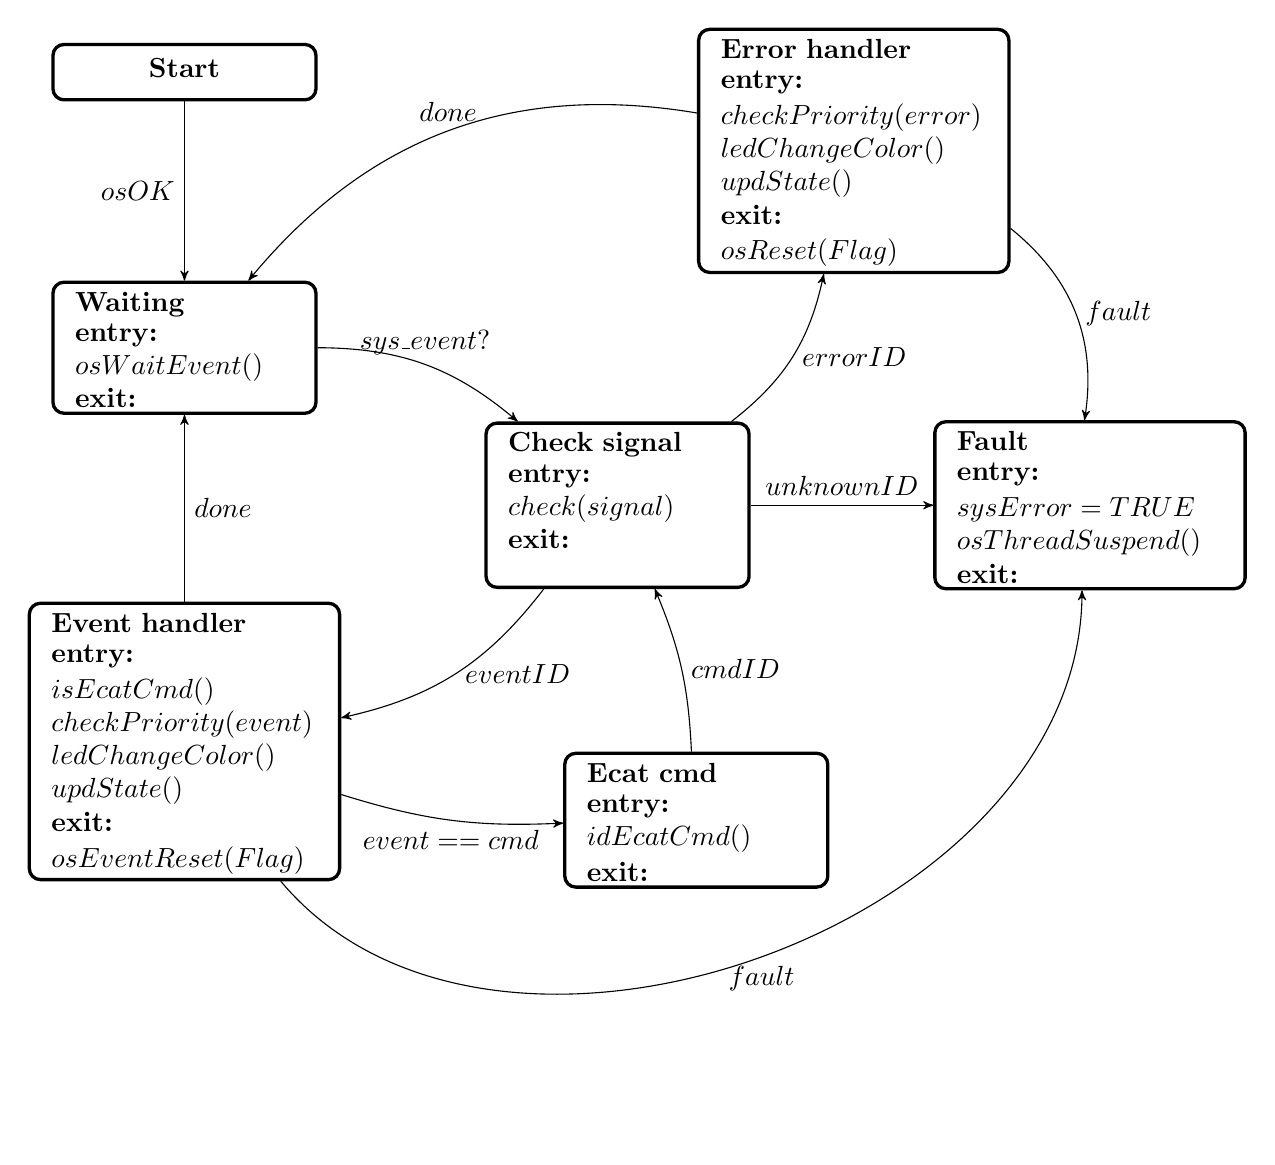
\begin{tikzpicture}[->,>=stealth']
        %   Event Handler
        % Position of Start 
        % Use previously defined 'state' as layout (see above)
        % use tabular for content to get columns/rows
        % parbox to limit width of the listing
        \node[state,
            text width=3.2cm 	
            ] (EV_START) 
        {
            \begin{tabular}{l}
            \textbf{Start}\\[.1em]
            
        \end{tabular}
        };
    
      % STATE E_WAIT
      \node[state,
      text width=3.2cm,
          below of=EV_START,
          %yshift=-2cm,
          node distance=3.5cm, 
          anchor=center ] (EV_WAIT) 
        {
          \begin{tabular}{l}
          \textbf{Waiting}\\[.1em]
          \parbox{3cm}{
              \textbf{entry:}\\
              $osWaitEvent()$\\
              \textbf{exit:}
              }
      \end{tabular}
      };
    
        % State: Check
        \node[state,    	% layout (defined above)
            text width=3.2cm, 	% max text width
            yshift=-2cm, 		% move 2cm in y
            xshift=1cm,
            right of=EV_WAIT, 	% Position is to the right of QUERY
            node distance=4.5cm, 	% distance to QUERY
            anchor=center] (EV_CHCK) 	% posistion relative to the center of the 'box'
        {%
        \begin{tabular}{l} 	% content
            \textbf{Check signal}\\[.1em]
            \parbox{2.8cm}{
                \textbf{entry:}\\
                $check(signal)$\\
                \textbf{exit:}\\
                }
        \end{tabular}
        };
    
        % STATE EV_FAULT
        \node[state,
            text width=3.8cm,
            right of=EV_CHCK,
            xshift=1.5cm,
            node distance=4.5cm,
            anchor=center] (EV_FAULT) 
        {%
        \begin{tabular}{l}
        \textbf{Fault}\\[.1em]
        \parbox{4cm}{
            \textbf{entry:}\\[.1em]
            $sysError = TRUE$\\
            $osThreadSuspend()$\\
            \textbf{exit:}
            }
        \end{tabular}
        };
    
        % STATE ERROR HANDLER
        % Use previously defined 'state' as layout (see above)
        % use tabular for content to get columns/rows
        % parbox to limit width of the listing
        \node[state,
            text width=3.8cm,
            above of = EV_CHCK,
            xshift = 3cm,
            yshift = 1cm,
            node distance = 3.5cm,
            anchor = center] (EV_HANDLER_ERROR) 
        {\begin{tabular}{l}
            \textbf{Error handler}\\[.1em]
            \parbox{4cm}{
                \textbf{entry:}\\[.1em]
                $checkPriority(error)$\\
                $ledChangeColor()$\\
                $updState()$\\
                \textbf{exit:}\\[.1em]
                $osReset(Flag)$
                } 
        \end{tabular}};
    
        % STATE EVENT HANDLER
        % Use previously defined 'state' as layout (see above)
        % use tabular for content to get columns/rows
        % parbox to limit width of the listing
        \node[state,
            text width=3.8cm,
            below of = EV_WAIT,
            %xshift = -3cm,
            yshift = -1.5cm,
            node distance = 3.5cm,
            anchor = center] (EV_HANDLER_EVENT) 
        {\begin{tabular}{l}
            \textbf{Event handler}\\[.1em]
            \parbox{4cm}{
                \textbf{entry:}\\[.1em]
                $isEcatCmd()$
                $checkPriority(event)$\\
                $ledChangeColor()$\\
                $updState()$\\
                \textbf{exit:}\\[.1em]
                $osEventReset(Flag)$
                } 
        \end{tabular}};
            
    
        %STATE ECAT CMD
        \node[state,
        text width = 3.2cm,
        below of=EV_CHCK,
        yshift= 0.5cm,
        xshift = 1cm,
        node distance=4.5cm,
        anchor=center] (EV_ECATCMD) 
        {%
        \begin{tabular}{l}
        \textbf{Ecat cmd}\\[.1em]
        \parbox{4cm}{
            \textbf{entry:}\\
            $idEcatCmd()$\\[.1em]
            \textbf{exit:}
            }
        \end{tabular}
        };
    
        % EV_START
        % EV_WAIT
        % EV_CHCK
        % EV_FAULT
        % EV_HANDLER_ERROR
        % EV_HANDLER_EVENT
        % EV_ECATCMD
        % draw the paths and and print some Text below/above the graph
        \path
            (EV_START)       edge node[anchor=center,left]{$osOK$}  (EV_WAIT) 
            (EV_WAIT) 	    edge[bend left=20]  node[anchor=north,above]{$sys\_event?$} (EV_CHCK)
            (EV_CHCK)     	edge[bend right=20] node[anchor=north,right]{$errorID$} (EV_HANDLER_ERROR)
            (EV_CHCK)       	edge  node[anchor=center,above]{$unknownID$}     (EV_FAULT)
            (EV_CHCK)       	edge[bend left=20] node[anchor=center,right]{$eventID$}   (EV_HANDLER_EVENT)
            % (E_CONNECTED)   edge            node[anchor=north,above]{$soes$}     
            %                                 node[anchor=south,below]{$timeout$}(E_FAULT)
            (EV_HANDLER_ERROR)   edge[bend right=30]  node[anchor=center,above]{$done$}   (EV_WAIT)
            (EV_HANDLER_ERROR)   edge[bend left=30]  node[anchor=center,right]{$fault$}   (EV_FAULT)
            % (E_FAULT)  	    edge            node[anchor=north,above]{$thread$} 
            %                                 node[anchor=center,below]{$removed?$}   (E_RESTART)
            (EV_HANDLER_EVENT)  	edge  node[anchor=center,right]{$done$}     (EV_WAIT)
            (EV_HANDLER_EVENT)  	edge[bend right=10] node[anchor=center,below]{$event==cmd$}(EV_ECATCMD)     
                                                        %node[anchor=center,below]{$==cmd$}
            (EV_HANDLER_EVENT)  	edge[bend right=70] node[anchor=center,below]{$fault$}     (EV_FAULT)
            (EV_ECATCMD)  	edge[bend right=10]  node[anchor=center,right]{$cmdID$}     (EV_CHCK)
            ;
    
        \end{tikzpicture}
    \caption{State machine for Event Handler functionality.}
    \label{fig:sm_event}
\end{figure}





%LED DSM
\begin{figure}[ht]
    \centering
    %Her comes the figure
    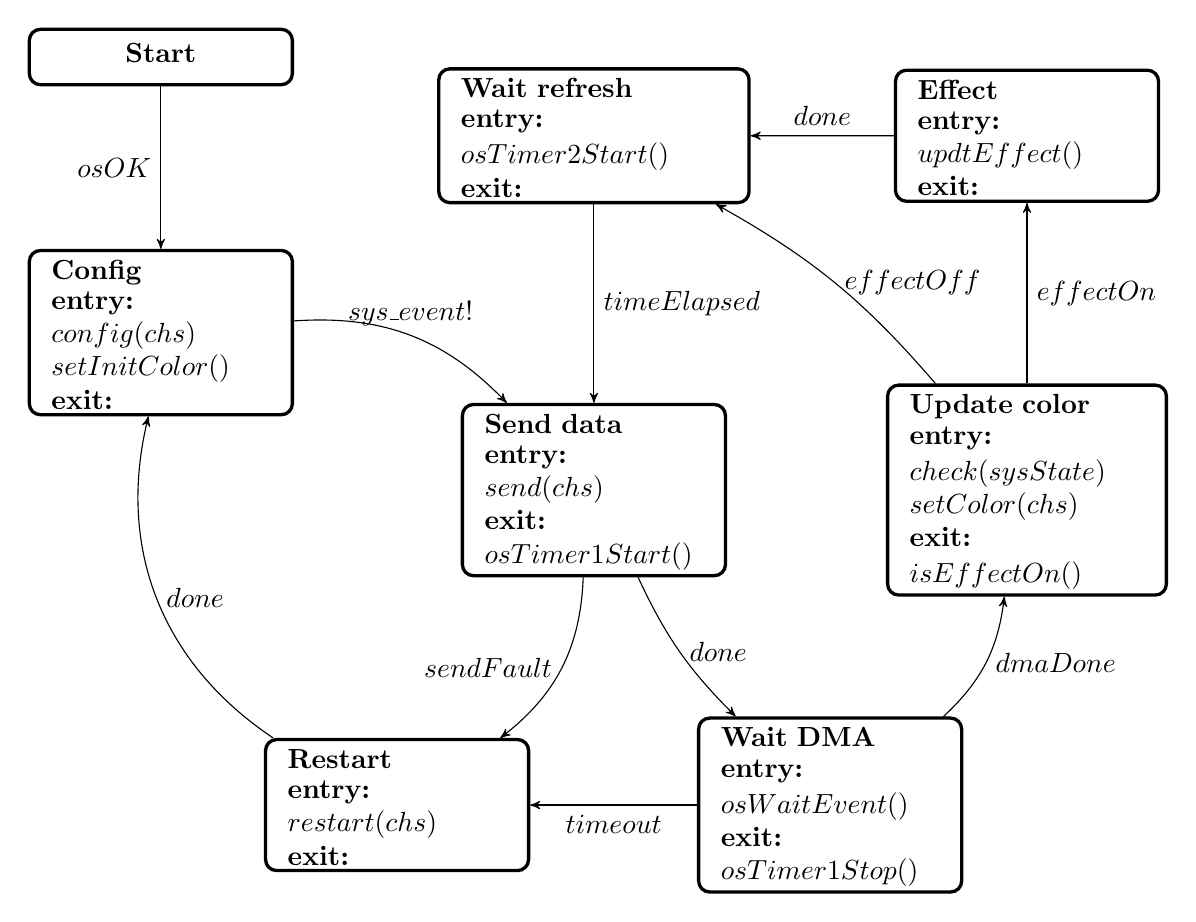
\begin{tikzpicture}[->,>=stealth']
        %   LED DSM
        % Position of Start 
        % Use previously defined 'state' as layout (see above)
        % use tabular for content to get columns/rows
        % parbox to limit width of the listing
        \node[state,
            text width=3.2cm 	
            ] (L_START) 
        {
            \begin{tabular}{l}
            \textbf{Start}\\[.1em]
            
        \end{tabular}
        };
    
      % STATE L_CONFIG
      \node[state,
      text width=3.2cm,
          below of=L_START,
          %yshift=-2cm,
          node distance=3.5cm, 
          anchor=center ] (L_CONFIG) 
        {
          \begin{tabular}{l}
          \textbf{Config}\\[.1em]
          \parbox{3cm}{
              \textbf{entry:}\\
              $config(chs)$\\
              $setInitColor()$
              \textbf{exit:}
              }
      \end{tabular}
      };
    
    
        % State: L_SEND
        \node[state,    	% layout (defined above)
            text width=3.2cm, 	% max text width
            yshift=-2cm, 		% move 2cm in y
            xshift=1cm,
            right of=L_CONFIG, 	% Position is to the right of QUERY
            node distance=4.5cm, 	% distance to QUERY
            anchor=center] (L_SEND) 	% posistion relative to the center of the 'box'
        {%
        \begin{tabular}{l} 	% content
            \textbf{Send data}\\[.1em]
            \parbox{2.8cm}{
                \textbf{entry:}\\
                $send(chs)$\\
                \textbf{exit:}\\
                $osTimer1Start()$
                }
        \end{tabular}
        };
    
        % STATE L_WAIT_REFRESH
        \node[state,
            text width=3.8cm,
            above of=L_SEND,
            %xshift=1.5cm,
            node distance=4.5cm,
            anchor=center] (L_WAIT_REFRESH) 
        {%
        \begin{tabular}{l}
        \textbf{Wait refresh}\\[.1em]
        \parbox{4cm}{
            \textbf{entry:}\\[.1em]
            $osTimer2Start()$\\
            \textbf{exit:}
            }
        \end{tabular}
        };
    
    
    
    
        % STATE L_C_UPDATE
        % Use previously defined 'state' as layout (see above)
        % use tabular for content to get columns/rows
        % parbox to limit width of the listing
        \node[state,
            text width=3.4cm,
            right of = L_SEND,
            xshift = 1cm,
            %yshift = -1.5cm,
            node distance = 4.5cm,
            anchor = center] (L_C_UPDATE) 
        {\begin{tabular}{l}
            \textbf{Update color}\\[.1em]
            \parbox{4cm}{
                \textbf{entry:}\\[.1em]
                $check(sysState)$
                $setColor(chs)$\\
                \textbf{exit:}\\[.1em]
                $isEffectOn()$
                } 
        \end{tabular}};
    
    
        % STATE 
        % Use previously defined 'state' as layout (see above)
        % use tabular for content to get columns/rows
        % parbox to limit width of the listing
        \node[state,
            text width=3.2cm,
            below of = L_C_UPDATE,
            xshift = -2.5cm,
            %yshift = -3.5cm,
            node distance = 4cm,
            anchor = center] (L_WAIT_DMA) 
        {\begin{tabular}{l}
            \textbf{Wait DMA}\\[.1em]
            \parbox{4cm}{
                \textbf{entry:}\\[.1em]
                $osWaitEvent()$\\
                \textbf{exit:}\\
                $osTimer1Stop()$
                } 
        \end{tabular}};
    
        %STATE L_EFFECT
        \node[state,
        text width = 3.2cm,
        above of=L_C_UPDATE,
        yshift= 1cm,
        %xshift = 1cm,
        node distance=3.5cm,
        anchor=center] (L_EFFECT) 
        {%
        \begin{tabular}{l}
        \textbf{Effect}\\[.1em]
        \parbox{4cm}{
            \textbf{entry:}\\
            $updtEffect()$\\
            \textbf{exit:}
            }
        \end{tabular}
        };
    
            %STATE L_RESTART
        \node[state,
        text width = 3.2cm,
        below of=L_SEND,
        %yshift= 0.5cm,
        xshift = -2.5cm,
        node distance=4cm,
        anchor=center] (L_RESTART) 
        {%
        \begin{tabular}{l}
        \textbf{Restart}\\[.1em]
        \parbox{4cm}{
            \textbf{entry:}\\
            $restart(chs)$\\
            \textbf{exit:}
            }
        \end{tabular}
        };
    
        % L_START
        % L_CONFIG
        % L_WAIT_DMA
        % L_SEND
        % L_C_UPDATE
        % L_WAIT_REFRESH
        % L_EFFECT
        % L_RESTART  
    
        % draw the paths and and print some Text below/above the graph
        \path
            (L_START)       edge node[anchor=center,left]{$osOK$}  (L_CONFIG) 
            (L_CONFIG) 	    edge[bend left=25]  node[anchor=north,above]{$sys\_event!$} (L_SEND)
            (L_SEND)     	edge[bend right=10] node[anchor=north,right]{$done$} (L_WAIT_DMA)
            (L_WAIT_DMA)       	edge[bend right=20]  node[anchor=center,right]{$dmaDone$}     (L_C_UPDATE)
            (L_WAIT_DMA)       	edge  node[anchor=center,below]{$timeout$}     (L_RESTART)
            (L_C_UPDATE)       	edge[bend right=10] node[anchor=center,right]{$effectOff$}   (L_WAIT_REFRESH)
            (L_C_UPDATE)   edge node[anchor=center,right]{$effectOn$}   (L_EFFECT)
            (L_EFFECT)   edge  node[anchor=center,above]{$done$}   (L_WAIT_REFRESH)
            % (E_FAULT)  	    edge            node[anchor=north,above]{$thread$} 
            %                                 node[anchor=center,below]{$removed?$}   (E_RESTART)
            (L_WAIT_REFRESH)  	edge  node[anchor=center,right]{$timeElapsed$}     (L_SEND)
            % (L_SEND)  	edge[bend right=10] node[anchor=center,below]{$event==cmd$}(EV_ECATCMD)     
            %                                             %node[anchor=center,below]{$==cmd$}
            (L_SEND)  	edge[bend left=25] node[anchor=center,left]{$sendFault$}     (L_RESTART)
            (L_RESTART)  	edge[bend left=35]  node[anchor=center,right]{$done$}     (L_CONFIG)
            ;
    
        \end{tikzpicture}
    \caption{State machine for LED Ring control functionality}
    \label{fig:sm_led}
\end{figure}




\begin{figure}[ht]
    \centering
    \subfigure[Synchronization state machine]{\label{subfig:ecat_sm}{
        %General state machine 80/100
        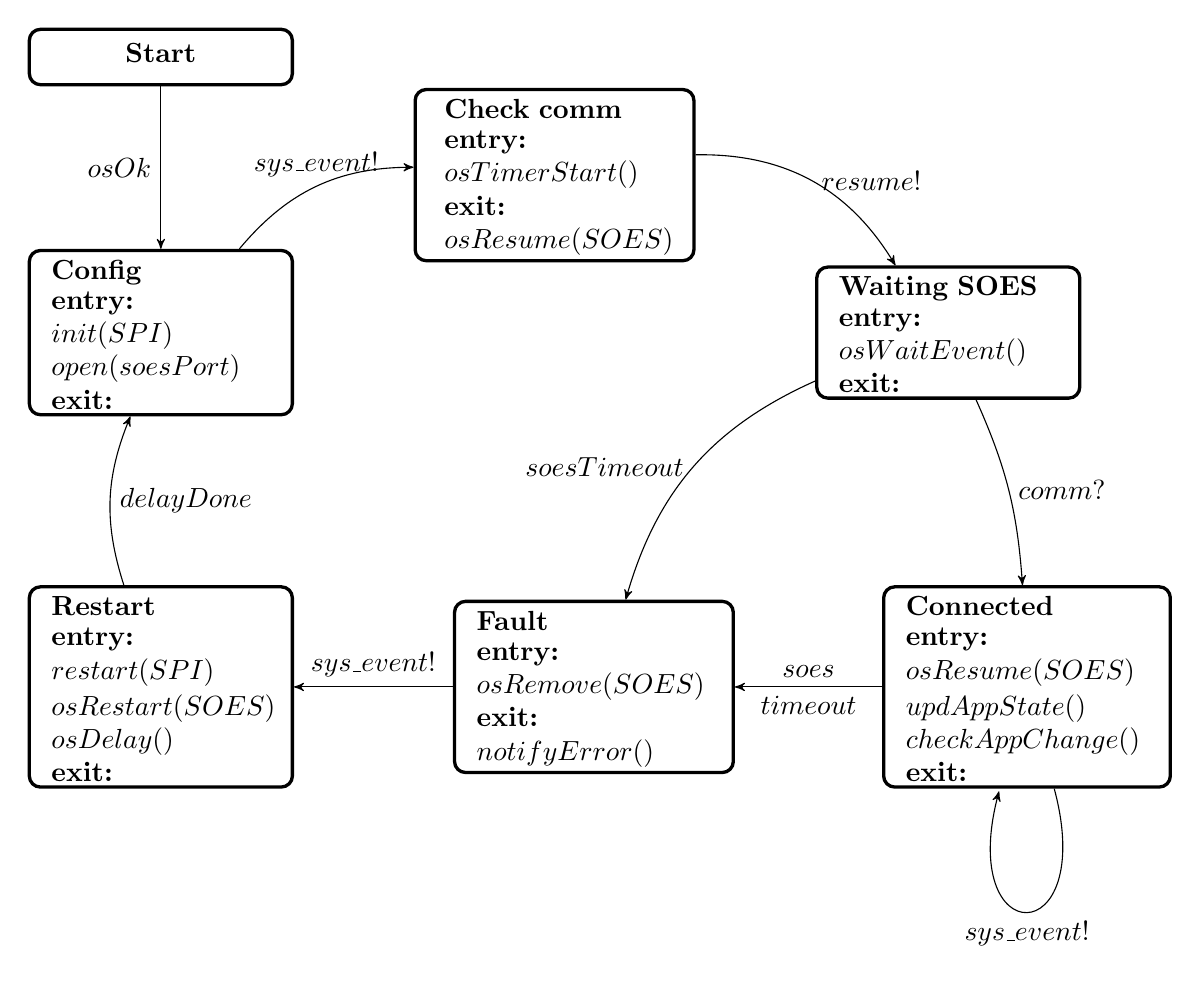
\begin{tikzpicture}[->,>=stealth']
        % Position of QUERY 
        % Use previously defined 'state' as layout (see above)
        % use tabular for content to get columns/rows
        % parbox to limit width of the listing
        \node[state,
            text width=3.2cm 	
            ] (E_CONFIG) 
        {\begin{tabular}{l}
            \textbf{Config}\\[.1em]
            \parbox{4cm}{
            \textbf{entry:}\\
            $init(SPI)$\\
            $open(soesPort)$\\
            \textbf{exit:}
            }
        \end{tabular}};
  
        % STATE START 
        % Use previously defined 'state' as layout (see above)
        % use tabular for content to get columns/rows
        % parbox to limit width of the listing
        \node[state,
            text width=3.2cm,
            above of = E_CONFIG,
            node distance = 3.5cm,
            anchor = center] (E_START) 
        {\begin{tabular}{l}
            \textbf{Start}\\[.1em]
            
        \end{tabular}};
  
  
            
        % State: ACK with different content
        \node[state,    	% layout (defined above)
            text width=3.4cm, 	% max text width
            yshift=2cm, 		% move 2cm in y
            right of=E_CONFIG, 	% Position is to the right of QUERY
            node distance=5cm, 	% distance to QUERY
            anchor=center] (E_CHCK) 	% posistion relative to the center of the 'box'
        {%
        \begin{tabular}{l} 	% content
            \textbf{Check comm}\\[.1em]
            \parbox{2.8cm}{
                \textbf{entry:}\\
                $osTimerStart()$
                \textbf{exit:}\\
                $osResume(SOES)$
                }
        \end{tabular}
        };
        
        % STATE E_WAIT
        \node[state,
        text width=3.2cm,
            %below of=ACK,
            right of=E_CHCK,
            yshift=-2cm,
            node distance=5cm, 
            anchor=center ] (E_WAIT) 
        {%
        \begin{tabular}{l}
            \textbf{Waiting SOES}\\[.1em]
            \parbox{2.8cm}{
                \textbf{entry:}\\
                $osWaitEvent()$\\
                \textbf{exit:}
                }
        \end{tabular}
        };
        
  
        
        %STATE CONNECTED
        \node[state,
        text width = 3.5cm,
        below of=E_WAIT,
        xshift= 1cm,
        node distance=4.5cm,
        anchor=center] (E_CONNECTED) 
        {%
        \begin{tabular}{l}
        \textbf{Connected}\\[.1em]
        \parbox{4cm}{
            \textbf{entry:}\\
            $osResume(SOES)$\\[.1em]
            $updAppState()$\\
            $checkAppChange()$\\
            \textbf{exit:}
            }
        \end{tabular}
        };
  
        % STATE E_FAULT
        \node[state,
            text width=3.4cm,
            left of=E_CONNECTED,
            %xshift=-2.5cm,
            node distance=5.5cm,
            anchor=center] (E_FAULT) 
        {%
        \begin{tabular}{l}
        \textbf{Fault}\\[.1em]
        \parbox{4cm}{
            \textbf{entry:}\\
            $osRemove(SOES)$\\
            \textbf{exit:}\\
            $notifyError()$
            }
        \end{tabular}
        };
  
        %STATE RESTART
        \node[state,
        text width = 3.2cm,
        left of=E_FAULT,
        node distance=5.5cm,
        %xshift = 2cm,
        anchor=center] (E_RESTART) 
        {%
        \begin{tabular}{l}
        \textbf{Restart}\\[.1em]
        \parbox{4cm}{
            \textbf{entry:}\\
            $restart(SPI)$\\[.1em]
            $osRestart(SOES)$\\
            $osDelay()$\\
            \textbf{exit:}
            }
        \end{tabular}
        };
  
        % draw the paths and and print some Text below/above the graph
        \path
            (E_START)       edge node[anchor=center,left]{$osOk$}  (E_CONFIG) 
            (E_CONFIG) 	    edge[bend left=25]  node[anchor=center,above]{$sys\_event!$} (E_CHCK)
            (E_CHCK)     	edge[bend left=30] node[anchor=north,right]{$resume!$} (E_WAIT)
            (E_WAIT)       	edge[bend left=10]  node[anchor=center,right]{$comm?$}     (E_CONNECTED)
            (E_WAIT)       	edge[bend right=25] node[anchor=center,left]{$soesTimeout$}                                         (E_FAULT)
            (E_CONNECTED)   edge            node[anchor=north,above]{$soes$}     
                                            node[anchor=south,below]{$timeout$}(E_FAULT)
            (E_CONNECTED)   edge[loop below]  node[anchor=left,below]{$sys\_event!$}                   (E_CONNECTED)
            (E_FAULT)  	    edge            node[anchor=north,above]{$sys\_event!$} (E_RESTART)
            %                                node[anchor=center,below]{$removed?$}   (E_RESTART)
            (E_RESTART)  	edge[bend left=20]  node[anchor=center,right]{$delayDone$}                                          (E_CONFIG)
            ;
  
        \end{tikzpicture}
    }}\hfill
    \subfigure[SOES application state machine]{\label{subfig:soes_sm}{
        %SOES state machine 80/100
        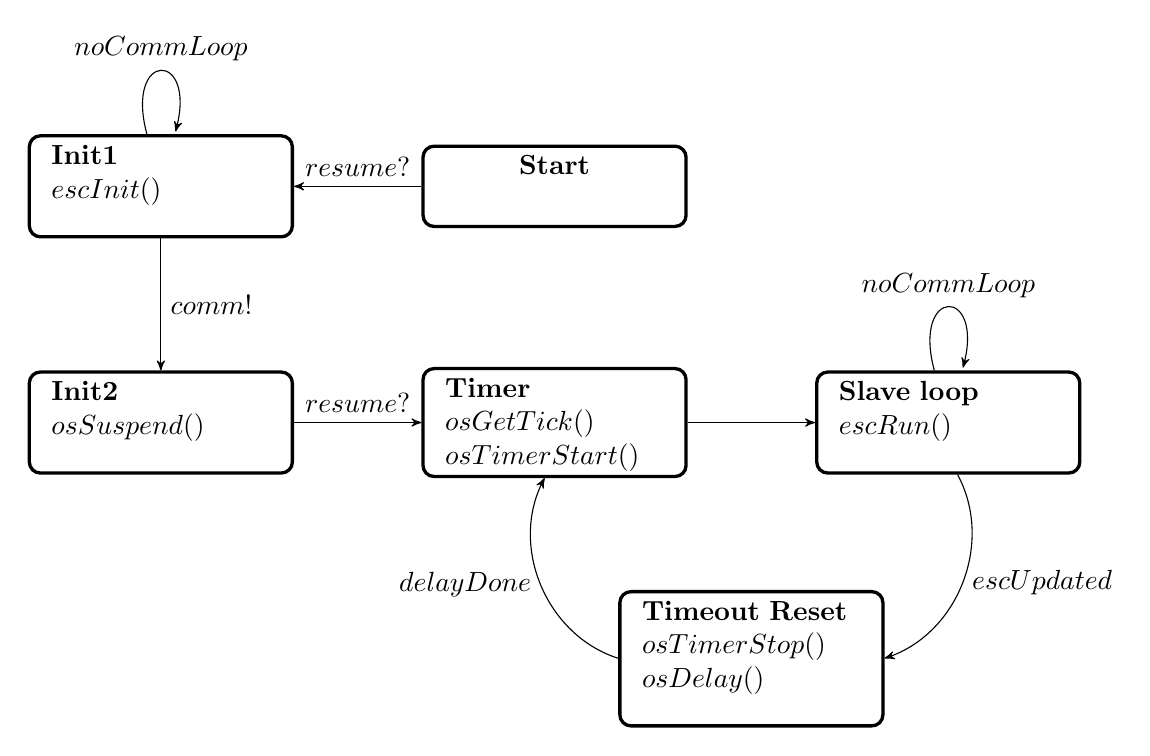
\begin{tikzpicture}[->,>=stealth']
        % STATE 1 SOES
        % Use previously defined 'state' as layout (see above)
        % use tabular for content to get columns/rows
        % parbox to limit width of the listing
        \node[state,
            text width=3.2cm 	
            ] (SOES_INIT1) 
        {\begin{tabular}{l}
            \textbf{Init1}\\[.1em]
            \parbox{4cm}{
            
            $escInit()$\\
            
            }
        \end{tabular}};
            
        % STATE SOES INIT 2
        \node[state,    	% layout (defined above)
            text width=3.2cm, 	% max text width
            %yshift=2cm, 		% move 2cm in y
            below of=SOES_INIT1, 	
            node distance=3cm, 	% 
            anchor=center] (SOES_INIT2) 	% posistion relative to the center of the 'box'
        {%
        \begin{tabular}{l} 	% content
            \textbf{Init2}\\[.1em]
            \parbox{2.8cm}{
                $osSuspend()$\\
                }
        \end{tabular}
        };
  
        % STATE 0 SOES
        % Use previously defined 'state' as layout (see above)
        % use tabular for content to get columns/rows
        % parbox to limit width of the listing
        \node[state,
            text width=3.2cm,
            right of = SOES_INIT1,
            node distance = 5cm,
            anchor = center] (SOES_INIT0) 
        {\begin{tabular}{l}
            \textbf{Start}\\[.1em]
            \parbox{4cm}{
            
            }
        \end{tabular}};
        
        % STATE SET TIMER
        \node[state,
        text width=3.2cm,
            %below of=ACK,
            right of=SOES_INIT2,
            %yshift=-2cm,
            node distance=5cm, 
            anchor=center ] (SOES_TIMER) 
        {%
        \begin{tabular}{l}
            \textbf{Timer}\\[.1em]
            \parbox{2.8cm}{
                $osGetTick()$\\
                $osTimerStart()$
                }
        \end{tabular}
        };
        
  
        
        %STATE SLAVE LOOP
        \node[state,
        text width = 3.2cm,
        right of=SOES_TIMER,
        %xshift= 2.5cm,
        node distance=5cm,
        anchor=center] (SOES_SLAVE) 
        {%
        \begin{tabular}{l}
        \textbf{Slave loop}\\[.1em]
        \parbox{4cm}{
            $escRun()$\\
            }
        \end{tabular}
        };
  
        % STATE SOES_RESET TIMEOUT
        \node[state,
            text width=3.2cm,
            below of=SOES_SLAVE,
            xshift=-2.5cm,
            node distance=3cm,
            anchor=center] (SOES_RESET) 
        {%
        \begin{tabular}{l}
        \textbf{Timeout Reset}\\[.1em]
        \parbox{4cm}{
            $osTimerStop()$\\
            $osDelay()$\\
            }
        \end{tabular}
        };
  
        
        draw the paths and and print some Text below/above the graph
        \path
        (SOES_INIT0)    edge node[anchor=center,above]{$resume?$} (SOES_INIT1) 
        (SOES_INIT1) 	edge  node[anchor=south,right]{$comm!$}  (SOES_INIT2)
        (SOES_INIT1)    edge [loop above]   node[anchor=east,above]{$noCommLoop$} (SOES_INIT1)
        (SOES_INIT2)    edge node [anchor=center,above]{$resume?$} (SOES_TIMER)                                          (SOES_TIMER)
        (SOES_TIMER)    edge                   (SOES_SLAVE)
        (SOES_SLAVE)    edge [loop above]       node[anchor=center,above]{$noCommLoop$}       (SOES_SLAVE)
        (SOES_SLAVE)    edge [bend left = 50]   node[anchor=center,right]{$escUpdated$}   (SOES_RESET)
        (SOES_RESET)    edge [bend left = 50]   node[anchor=center,left]{$delayDone$}   (SOES_TIMER)
        ;
  
        \end{tikzpicture}
    }}
    \caption{State machines for EtherCAT slave functionality.} %EtherCAT Device Protocol poster from EtherCAT resources
    \label{fig:sm_ecatsoes}
  \end{figure} 

% \begin{figure}[ht]
%     \centering
%     \subfigure[Synchronization state machine]{\label{subfig:ecat_sm}{
%         %General state machine 80/100
%         \begin{tikzpicture}[->,>=stealth']
%         % Position of QUERY 
%         % Use previously defined 'state' as layout (see above)
%         % use tabular for content to get columns/rows
%         % parbox to limit width of the listing
%         \node[state,
%             text width=3.2cm 	
%             ] (E_CONFIG) 
%         {\begin{tabular}{l}
%             \textbf{Config}\\[.1em]
%             \parbox{4cm}{
%             \textbf{entry:}\\
%             $spi\_init()$\\
%             $open\_soesPort()$\\
%             \textbf{exit:}
%             }
%         \end{tabular}};

%         % STATE START 
%         % Use previously defined 'state' as layout (see above)
%         % use tabular for content to get columns/rows
%         % parbox to limit width of the listing
%         \node[state,
%             text width=3.2cm,
%             above of = E_CONFIG,
%             node distance = 3.5cm,
%             anchor = center] (E_START) 
%         {\begin{tabular}{l}
%             \textbf{Start}\\[.1em]
            
%         \end{tabular}};


            
%         % State: ACK with different content
%         \node[state,    	% layout (defined above)
%             text width=3.2cm, 	% max text width
%             yshift=2cm, 		% move 2cm in y
%             right of=E_CONFIG, 	% Position is to the right of QUERY
%             node distance=5cm, 	% distance to QUERY
%             anchor=center] (E_CHCK) 	% posistion relative to the center of the 'box'
%         {%
%         \begin{tabular}{l} 	% content
%             \textbf{Check comm}\\[.1em]
%             \parbox{2.8cm}{
%                 \textbf{entry:}\\
%                 $timeout\_start()$
%                 \textbf{exit:}\\
%                 $resume\_SOES()$
%                 }
%         \end{tabular}
%         };
        
%         % STATE E_WAIT
%         \node[state,
%         text width=3.2cm,
%             %below of=ACK,
%             right of=E_CHCK,
%             yshift=-2cm,
%             node distance=5cm, 
%             anchor=center ] (E_WAIT) 
%         {%
%         \begin{tabular}{l}
%             \textbf{Waiting SOES}\\[.1em]
%             \parbox{2.8cm}{
%                 \textbf{entry:}\\
%                 $osWaitEvent()$\\
%                 \textbf{exit:}
%                 }
%         \end{tabular}
%         };
        

        
%         %STATE CONNECTED
%         \node[state,
%         text width = 3.2cm,
%         below of=E_WAIT,
%         xshift= 2.5cm,
%         node distance=4.5cm,
%         anchor=center] (E_CONNECTED) 
%         {%
%         \begin{tabular}{l}
%         \textbf{Connected}\\[.1em]
%         \parbox{4cm}{
%             \textbf{entry:}\\
%             $osResume(SOES)$\\[.1em]
%             $update\_state()$\\
%             \textbf{exit:}
%             }
%         \end{tabular}
%         };

%         % STATE E_FAULT
%         \node[state,
%             text width=3.2cm,
%             below of=E_WAIT,
%             xshift=-2.5cm,
%             node distance=4.5cm,
%             anchor=center] (E_FAULT) 
%         {%
%         \begin{tabular}{l}
%         \textbf{Fault}\\[.1em]
%         \parbox{4cm}{
%             \textbf{entry:}\\
%             $notify\_error()$\\
%             $osThreadRemove()$\\
%             \textbf{exit:}
%             }
%         \end{tabular}
%         };

%         %STATE RESTART
%         \node[state,
%         text width = 3.2cm,
%         left of=E_FAULT,
%         node distance=5cm,
%         %xshift = 2cm,
%         anchor=center] (E_RESTART) 
%         {%
%         \begin{tabular}{l}
%         \textbf{Restart}\\[.1em]
%         \parbox{4cm}{
%             \textbf{entry:}\\
%             $deInit_SPI()$\\[.1em]
%             $restartSOES$\\
%             $delay()$
%             }
%         \end{tabular}
%         };

%         % draw the paths and and print some Text below/above the graph
%         \path
%             (E_START)       edge node[anchor=center,left]{$os\_ready$}  (E_CONFIG) 
%             (E_CONFIG) 	    edge[bend left=20]  node[anchor=north,above]{$port\_ok$} (E_CHCK)
%             (E_CHCK)     	edge[bend left=20] node[anchor=north,right]{$Resume!$} (E_WAIT)
%             (E_WAIT)       	edge[bend left=10]  node[anchor=center,right]{$Comm?$}     (E_CONNECTED)
%             (E_WAIT)       	edge[bend right=10] node[anchor=center,left]{$soes\_timeout$}                                         (E_FAULT)
%             (E_CONNECTED)   edge            node[anchor=north,above]{$soes$}     
%                                             node[anchor=south,below]{$timeout$}(E_FAULT)
%             (E_CONNECTED)   edge[loop below]  node[anchor=center,below]{$update\_loop$}                   (E_CONNECTED)
%             (E_FAULT)  	    edge            node[anchor=north,above]{$thread$} 
%                                             node[anchor=center,below]{$removed?$}   (E_RESTART)
%             (E_RESTART)  	edge[bend left=30]  node[anchor=center,left]{$delay\_done$}                                          (E_CONFIG)
%             ;

%         \end{tikzpicture}
%     }}\hfill
%     \subfigure[SOES application state machine]{\label{subfig:soes_sm}{
%         %SOES state machine 80/100
%         \begin{tikzpicture}[->,>=stealth']
%         % STATE 1 SOES
%         % Use previously defined 'state' as layout (see above)
%         % use tabular for content to get columns/rows
%         % parbox to limit width of the listing
%         \node[state,
%             text width=3.2cm 	
%             ] (SOES_INIT1) 
%         {\begin{tabular}{l}
%             \textbf{Init1}\\[.1em]
%             \parbox{4cm}{
            
%             $lib\_init()$\\
            
%             }
%         \end{tabular}};
            
%         % STATE SOES INIT 2
%         \node[state,    	% layout (defined above)
%             text width=3.2cm, 	% max text width
%             %yshift=2cm, 		% move 2cm in y
%             below of=SOES_INIT1, 	
%             node distance=3cm, 	% 
%             anchor=center] (SOES_INIT2) 	% posistion relative to the center of the 'box'
%         {%
%         \begin{tabular}{l} 	% content
%             \textbf{Init2}\\[.1em]
%             \parbox{2.8cm}{
%                 $suspend\_thread()$\\
%                 }
%         \end{tabular}
%         };

%         % STATE 0 SOES
%         % Use previously defined 'state' as layout (see above)
%         % use tabular for content to get columns/rows
%         % parbox to limit width of the listing
%         \node[state,
%             text width=3.2cm,
%             right of = SOES_INIT1,
%             node distance = 5cm,
%             anchor = center] (SOES_INIT0) 
%         {\begin{tabular}{l}
%             \textbf{Start}\\[.1em]
%             \parbox{4cm}{
            
%             }
%         \end{tabular}};
        
%         % STATE SET TIMER
%         \node[state,
%         text width=3.2cm,
%             %below of=ACK,
%             right of=SOES_INIT2,
%             %yshift=-2cm,
%             node distance=5cm, 
%             anchor=center ] (SOES_TIMER) 
%         {%
%         \begin{tabular}{l}
%             \textbf{Timer}\\[.1em]
%             \parbox{2.8cm}{
%                 $osGetTick()$\\
%                 $osStartTimeout()$
%                 }
%         \end{tabular}
%         };
        

        
%         %STATE SLAVE LOOP
%         \node[state,
%         text width = 3.2cm,
%         right of=SOES_TIMER,
%         %xshift= 2.5cm,
%         node distance=5cm,
%         anchor=center] (SOES_SLAVE) 
%         {%
%         \begin{tabular}{l}
%         \textbf{Slave loop}\\[.1em]
%         \parbox{4cm}{
%             $eca\_slv()$\\
%             }
%         \end{tabular}
%         };

%         % STATE SOES_RESET TIMEOUT
%         \node[state,
%             text width=3.2cm,
%             below of=SOES_SLAVE,
%             xshift=-2.5cm,
%             node distance=3cm,
%             anchor=center] (SOES_RESET) 
%         {%
%         \begin{tabular}{l}
%         \textbf{Timeout Reset}\\[.1em]
%         \parbox{4cm}{
%             $reset\_Timeout()$\\
%             $osDelay()$\\
%             }
%         \end{tabular}
%         };

        
%         draw the paths and and print some Text below/above the graph
%         \path
%         (SOES_INIT0)    edge node[anchor=center,above]{$Resume?$} (SOES_INIT1) 
%         (SOES_INIT1) 	edge  node[anchor=south,right]{$Comm!$}  (SOES_INIT2)
%         (SOES_INIT1)    edge [loop above]   node[anchor=east,above]{$no\_comm\_loop$} (SOES_INIT1)
%         (SOES_INIT2)    edge [loop below]   node[anchor=south,below]{$no\_eventFlag$} (SOES_INIT2)
%         (SOES_INIT2)    edge node [anchor=center,above]{$Resume?$} (SOES_TIMER)                                          (SOES_TIMER)
%         (SOES_TIMER)    edge                   (SOES_SLAVE)
%         (SOES_SLAVE)    edge [loop above]       node[anchor=center,above]{$no\_comm\_loop$}       (SOES_SLAVE)
%         (SOES_SLAVE)    edge [bend left = 50]   node[anchor=center,right]{$esc\_updated$}   (SOES_RESET)
%         (SOES_RESET)    edge [bend left = 50]   node[anchor=center,left]{$delay\_done$}   (SOES_TIMER)
%         ;

%         \end{tikzpicture}
%     }}
%     \caption{State machines for EtherCAT slave functionality} %EtherCAT Device Protocol poster from EtherCAT resources
%     \label{fig:syncmodes}
% \end{figure} 

% \begin{figure}[ht]
%     \centering
%     %Her comes the figure
%     \caption{This is a figure}
%     \label{fig:this_is_a_label}
% \end{figure}

% The End
\end{document}


